\documentclass[1p]{elsarticle_modified}
%\bibliographystyle{elsarticle-num}

%\usepackage[colorlinks]{hyperref}
%\usepackage{abbrmath_seonhwa} %\Abb, \Ascr, \Acal ,\Abf, \Afrak
\usepackage{amsfonts}
\usepackage{amssymb}
\usepackage{amsmath}
\usepackage{amsthm}
\usepackage{scalefnt}
\usepackage{amsbsy}
\usepackage{kotex}
\usepackage{caption}
\usepackage{subfig}
\usepackage{color}
\usepackage{graphicx}
\usepackage{xcolor} %% white, black, red, green, blue, cyan, magenta, yellow
\usepackage{float}
\usepackage{setspace}
\usepackage{hyperref}

\usepackage{tikz}
\usetikzlibrary{arrows}

\usepackage{multirow}
\usepackage{array} % fixed length table
\usepackage{hhline}

%%%%%%%%%%%%%%%%%%%%%
\makeatletter
\renewcommand*\env@matrix[1][\arraystretch]{%
	\edef\arraystretch{#1}%
	\hskip -\arraycolsep
	\let\@ifnextchar\new@ifnextchar
	\array{*\c@MaxMatrixCols c}}
\makeatother %https://tex.stackexchange.com/questions/14071/how-can-i-increase-the-line-spacing-in-a-matrix
%%%%%%%%%%%%%%%

\usepackage[normalem]{ulem}

\newcommand{\msout}[1]{\ifmmode\text{\sout{\ensuremath{#1}}}\else\sout{#1}\fi}
%SOURCE: \msout is \stkout macro in https://tex.stackexchange.com/questions/20609/strikeout-in-math-mode

\newcommand{\cancel}[1]{
	\ifmmode
	{\color{red}\msout{#1}}
	\else
	{\color{red}\sout{#1}}
	\fi
}

\newcommand{\add}[1]{
	{\color{blue}\uwave{#1}}
}

\newcommand{\replace}[2]{
	\ifmmode
	{\color{red}\msout{#1}}{\color{blue}\uwave{#2}}
	\else
	{\color{red}\sout{#1}}{\color{blue}\uwave{#2}}
	\fi
}

\newcommand{\Sol}{\mathcal{S}} %segment
\newcommand{\D}{D} %diagram
\newcommand{\A}{\mathcal{A}} %arc


%%%%%%%%%%%%%%%%%%%%%%%%%%%%%5 test

\def\sl{\operatorname{\textup{SL}}(2,\Cbb)}
\def\psl{\operatorname{\textup{PSL}}(2,\Cbb)}
\def\quan{\mkern 1mu \triangleright \mkern 1mu}

\theoremstyle{definition}
\newtheorem{thm}{Theorem}[section]
\newtheorem{prop}[thm]{Proposition}
\newtheorem{lem}[thm]{Lemma}
\newtheorem{ques}[thm]{Question}
\newtheorem{cor}[thm]{Corollary}
\newtheorem{defn}[thm]{Definition}
\newtheorem{exam}[thm]{Example}
\newtheorem{rmk}[thm]{Remark}
\newtheorem{alg}[thm]{Algorithm}

\newcommand{\I}{\sqrt{-1}}
\begin{document}

%\begin{frontmatter}
%
%\title{Boundary parabolic representations of knots up to 8 crossings}
%
%%% Group authors per affiliation:
%\author{Yunhi Cho} 
%\address{Department of Mathematics, University of Seoul, Seoul, Korea}
%\ead{yhcho@uos.ac.kr}
%
%
%\author{Seonhwa Kim} %\fnref{s_kim}}
%\address{Center for Geometry and Physics, Institute for Basic Science, Pohang, 37673, Korea}
%\ead{ryeona17@ibs.re.kr}
%
%\author{Hyuk Kim}
%\address{Department of Mathematical Sciences, Seoul National University, Seoul 08826, Korea}
%\ead{hyukkim@snu.ac.kr}
%
%\author{Seokbeom Yoon}
%\address{Department of Mathematical Sciences, Seoul National University, Seoul, 08826,  Korea}
%\ead{sbyoon15@snu.ac.kr}
%
%\begin{abstract}
%We find all boundary parabolic representation of knots up to 8 crossings.
%
%\end{abstract}
%\begin{keyword}
%    \MSC[2010] 57M25 
%\end{keyword}
%
%\end{frontmatter}

%\linenumbers
%\tableofcontents
%
\newcommand\colored[1]{\textcolor{white}{\rule[-0.35ex]{0.8em}{1.4ex}}\kern-0.8em\color{red} #1}%
%\newcommand\colored[1]{\textcolor{white}{ #1}\kern-2.17ex	\textcolor{white}{ #1}\kern-1.81ex	\textcolor{white}{ #1}\kern-2.15ex\color{red}#1	}

{\Large $\underline{12a_{0895}~(K12a_{0895})}$}

\setlength{\tabcolsep}{10pt}
\renewcommand{\arraystretch}{1.6}
\vspace{1cm}\begin{tabular}{m{100pt}>{\centering\arraybackslash}m{274pt}}
\multirow{5}{120pt}{
	\centering
	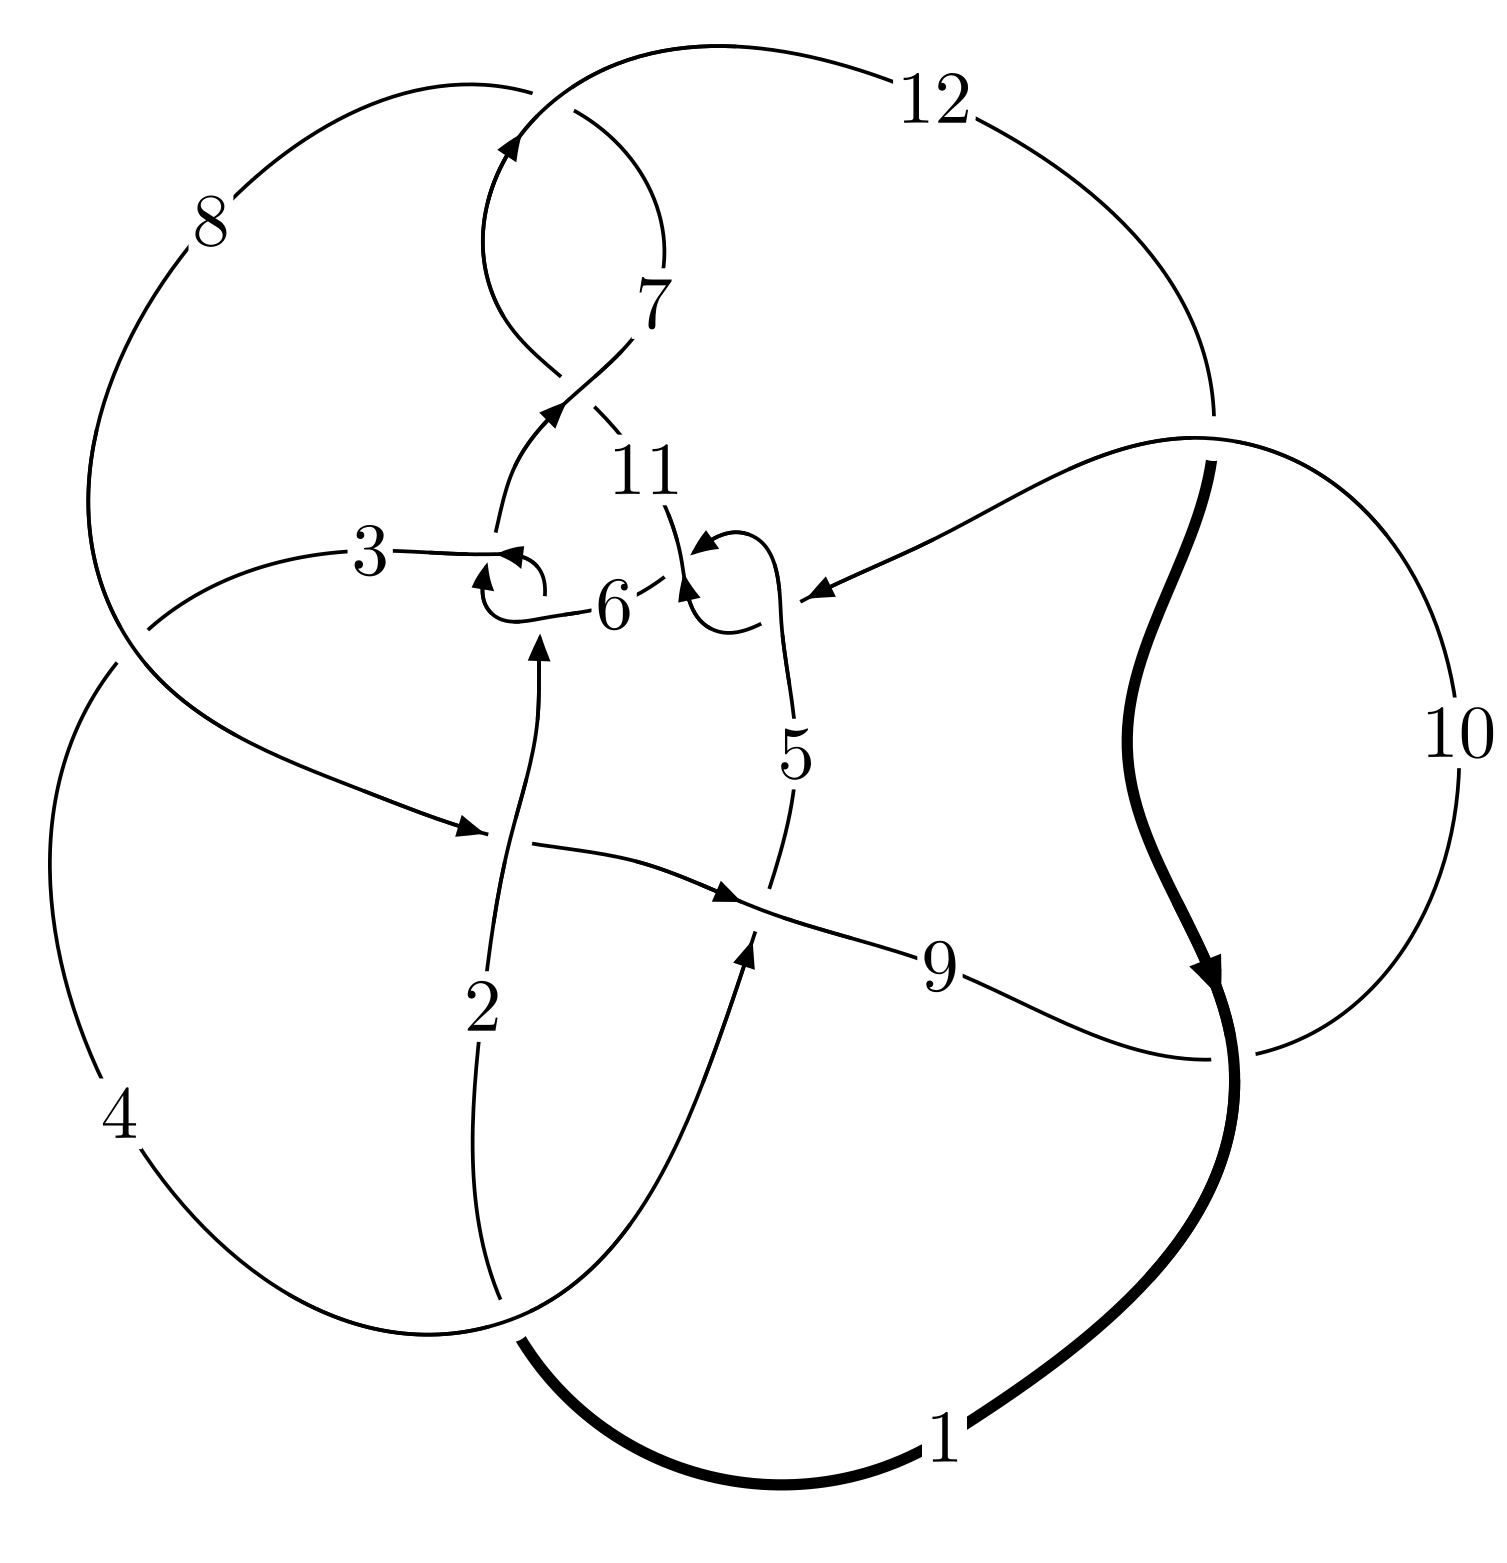
\includegraphics[width=112pt]{../../../GIT/diagram.site/Diagrams/png/1696_12a_0895.png}\\
\ \ \ A knot diagram\footnotemark}&
\allowdisplaybreaks
\textbf{Linearized knot diagam} \\
\cline{2-2}
 &
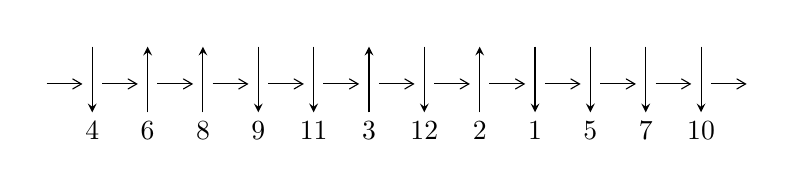
\begin{tikzpicture}[x=20pt, y=17pt]
	% nodes
	\node (C0) at (0, 0) {};
	\node (C1) at (1, 0) {};
	\node (C1U) at (1, +1) {};
	\node (C1D) at (1, -1) {4};

	\node (C2) at (2, 0) {};
	\node (C2U) at (2, +1) {};
	\node (C2D) at (2, -1) {6};

	\node (C3) at (3, 0) {};
	\node (C3U) at (3, +1) {};
	\node (C3D) at (3, -1) {8};

	\node (C4) at (4, 0) {};
	\node (C4U) at (4, +1) {};
	\node (C4D) at (4, -1) {9};

	\node (C5) at (5, 0) {};
	\node (C5U) at (5, +1) {};
	\node (C5D) at (5, -1) {11};

	\node (C6) at (6, 0) {};
	\node (C6U) at (6, +1) {};
	\node (C6D) at (6, -1) {3};

	\node (C7) at (7, 0) {};
	\node (C7U) at (7, +1) {};
	\node (C7D) at (7, -1) {12};

	\node (C8) at (8, 0) {};
	\node (C8U) at (8, +1) {};
	\node (C8D) at (8, -1) {2};

	\node (C9) at (9, 0) {};
	\node (C9U) at (9, +1) {};
	\node (C9D) at (9, -1) {1};

	\node (C10) at (10, 0) {};
	\node (C10U) at (10, +1) {};
	\node (C10D) at (10, -1) {5};

	\node (C11) at (11, 0) {};
	\node (C11U) at (11, +1) {};
	\node (C11D) at (11, -1) {7};

	\node (C12) at (12, 0) {};
	\node (C12U) at (12, +1) {};
	\node (C12D) at (12, -1) {10};
	\node (C13) at (13, 0) {};

	% arrows
	\draw[->,>={angle 60}]
	(C0) edge (C1) (C1) edge (C2) (C2) edge (C3) (C3) edge (C4) (C4) edge (C5) (C5) edge (C6) (C6) edge (C7) (C7) edge (C8) (C8) edge (C9) (C9) edge (C10) (C10) edge (C11) (C11) edge (C12) (C12) edge (C13) ;	\draw[->,>=stealth]
	(C1U) edge (C1D) (C2D) edge (C2U) (C3D) edge (C3U) (C4U) edge (C4D) (C5U) edge (C5D) (C6D) edge (C6U) (C7U) edge (C7D) (C8D) edge (C8U) (C9U) edge (C9D) (C10U) edge (C10D) (C11U) edge (C11D) (C12U) edge (C12D) ;
	\end{tikzpicture} \\
\hhline{~~} \\& 
\textbf{Solving Sequence} \\ \cline{2-2} 
 &
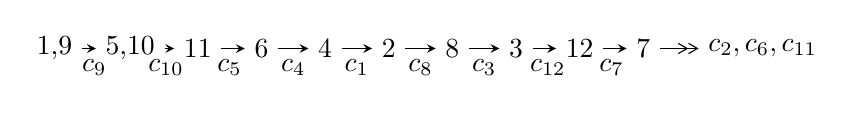
\begin{tikzpicture}[x=23pt, y=7pt]
	% node
	\node (A0) at (-1/8, 0) {1,9};
	\node (A1) at (17/16, 0) {5,10};
	\node (A2) at (17/8, 0) {11};
	\node (A3) at (25/8, 0) {6};
	\node (A4) at (33/8, 0) {4};
	\node (A5) at (41/8, 0) {2};
	\node (A6) at (49/8, 0) {8};
	\node (A7) at (57/8, 0) {3};
	\node (A8) at (65/8, 0) {12};
	\node (A9) at (73/8, 0) {7};
	\node (C1) at (1/2, -1) {$c_{9}$};
	\node (C2) at (13/8, -1) {$c_{10}$};
	\node (C3) at (21/8, -1) {$c_{5}$};
	\node (C4) at (29/8, -1) {$c_{4}$};
	\node (C5) at (37/8, -1) {$c_{1}$};
	\node (C6) at (45/8, -1) {$c_{8}$};
	\node (C7) at (53/8, -1) {$c_{3}$};
	\node (C8) at (61/8, -1) {$c_{12}$};
	\node (C9) at (69/8, -1) {$c_{7}$};
	\node (A10) at (11, 0) {$c_{2},c_{6},c_{11}$};

	% edge
	\draw[->,>=stealth]	
	(A0) edge (A1) (A1) edge (A2) (A2) edge (A3) (A3) edge (A4) (A4) edge (A5) (A5) edge (A6) (A6) edge (A7) (A7) edge (A8) (A8) edge (A9) ;
	\draw[->>,>={angle 60}]	
	(A9) edge (A10);
\end{tikzpicture} \\ 

\end{tabular} \\

\footnotetext{
The image of knot diagram is generated by the software ``\textbf{Draw programme}" developed by Andrew Bartholomew(\url{http://www.layer8.co.uk/maths/draw/index.htm\#Running-draw}), where we modified some parts for our purpose(\url{https://github.com/CATsTAILs/LinksPainter}).
}\phantom \\ \newline 
\centering \textbf{Ideals for irreducible components\footnotemark of $X_{\text{par}}$} 
 
\begin{align*}
I^u_{1}&=\langle 
-5.76967\times10^{713} u^{140}-2.01798\times10^{714} u^{139}+\cdots+5.49307\times10^{715} b-4.88700\times10^{716},\\
\phantom{I^u_{1}}&\phantom{= \langle  }-3.01897\times10^{716} u^{140}-1.28805\times10^{717} u^{139}+\cdots+4.46587\times10^{718} a+4.49215\times10^{719},\\
\phantom{I^u_{1}}&\phantom{= \langle  }u^{141}+4 u^{140}+\cdots+17088 u-2439\rangle \\
I^u_{2}&=\langle 
7.04074\times10^{51} u^{39}-4.76153\times10^{52} u^{38}+\cdots+1.87032\times10^{52} b+3.25362\times10^{52},\\
\phantom{I^u_{2}}&\phantom{= \langle  }-9.67601\times10^{51} u^{39}+7.48438\times10^{52} u^{38}+\cdots+1.87032\times10^{52} a+1.84688\times10^{53},\;u^{40}-7 u^{39}+\cdots- u+1\rangle \\
I^u_{3}&=\langle 
1.91827\times10^{15} u^{23}-1.49385\times10^{15} u^{22}+\cdots+6.45013\times10^{15} b-5.92118\times10^{16},\\
\phantom{I^u_{3}}&\phantom{= \langle  }-3.90530\times10^{16} u^{23}+3.28309\times10^{16} u^{22}+\cdots+7.09515\times10^{16} a+1.19578\times10^{18},\\
\phantom{I^u_{3}}&\phantom{= \langle  }u^{24}+6 u^{22}+\cdots-35 u+22\rangle \\
I^u_{4}&=\langle 
2 a u+5 b+4 a+2 u-1,\;2 a^2+a u+2 a+7,\;u^2+1\rangle \\
\\
\end{align*}
\raggedright * 4 irreducible components of $\dim_{\mathbb{C}}=0$, with total 209 representations.\\
\footnotetext{All coefficients of polynomials are rational numbers. But the coefficients are sometimes approximated in decimal forms when there is not enough margin.}
\newpage
\renewcommand{\arraystretch}{1}
\centering \section*{I. $I^u_{1}= \langle -5.77\times10^{713} u^{140}-2.02\times10^{714} u^{139}+\cdots+5.49\times10^{715} b-4.89\times10^{716},\;-3.02\times10^{716} u^{140}-1.29\times10^{717} u^{139}+\cdots+4.47\times10^{718} a+4.49\times10^{719},\;u^{141}+4 u^{140}+\cdots+17088 u-2439 \rangle$}
\flushleft \textbf{(i) Arc colorings}\\
\begin{tabular}{m{7pt} m{180pt} m{7pt} m{180pt} }
\flushright $a_{1}=$&$\begin{pmatrix}0\\u\end{pmatrix}$ \\
\flushright $a_{9}=$&$\begin{pmatrix}1\\0\end{pmatrix}$ \\
\flushright $a_{5}=$&$\begin{pmatrix}0.00676008 u^{140}+0.0288421 u^{139}+\cdots+29.7986 u-10.0588\\0.0105035 u^{140}+0.0367369 u^{139}+\cdots-98.0007 u+8.89665\end{pmatrix}$ \\
\flushright $a_{10}=$&$\begin{pmatrix}1\\u^2\end{pmatrix}$ \\
\flushright $a_{11}=$&$\begin{pmatrix}-0.00145415 u^{140}-0.0330147 u^{139}+\cdots-461.608 u+67.9518\\0.000487711 u^{140}+0.000914384 u^{139}+\cdots-29.1630 u+4.04438\end{pmatrix}$ \\
\flushright $a_{6}=$&$\begin{pmatrix}0.0698353 u^{140}+0.335805 u^{139}+\cdots+725.297 u-128.431\\-0.0172725 u^{140}-0.0588641 u^{139}+\cdots+170.894 u-17.6429\end{pmatrix}$ \\
\flushright $a_{4}=$&$\begin{pmatrix}0.0172636 u^{140}+0.0655790 u^{139}+\cdots-68.2021 u-1.16219\\0.0105035 u^{140}+0.0367369 u^{139}+\cdots-98.0007 u+8.89665\end{pmatrix}$ \\
\flushright $a_{2}=$&$\begin{pmatrix}0.0273329 u^{140}+0.108049 u^{139}+\cdots-59.1992 u+4.91525\\0.00133350 u^{140}+0.00670385 u^{139}+\cdots+22.2324 u-4.11296\end{pmatrix}$ \\
\flushright $a_{8}=$&$\begin{pmatrix}-0.00194108 u^{140}+0.0360596 u^{139}+\cdots+750.730 u-108.524\\0.000164712 u^{140}+0.000743466 u^{139}+\cdots+15.2249 u-1.76281\end{pmatrix}$ \\
\flushright $a_{3}=$&$\begin{pmatrix}0.106236 u^{140}+0.508300 u^{139}+\cdots+1272.99 u-219.614\\-0.00228481 u^{140}-0.000604315 u^{139}+\cdots+187.057 u-25.4958\end{pmatrix}$ \\
\flushright $a_{12}=$&$\begin{pmatrix}u\\u^3+u\end{pmatrix}$ \\
\flushright $a_{7}=$&$\begin{pmatrix}-0.00248641 u^{140}+0.0321432 u^{139}+\cdots+722.092 u-104.111\\-0.000299686 u^{140}-0.00101533 u^{139}+\cdots+14.9075 u-1.58172\end{pmatrix}$\\&\end{tabular}
\flushleft \textbf{(ii) Obstruction class $= -1$}\\~\\
\flushleft \textbf{(iii) Cusp Shapes $= 0.0414932 u^{140}+0.207190 u^{139}+\cdots+724.356 u-117.682$}\\~\\
\newpage\renewcommand{\arraystretch}{1}
\flushleft \textbf{(iv) u-Polynomials at the component}\newline \\
\begin{tabular}{m{50pt}|m{274pt}}
Crossings & \hspace{64pt}u-Polynomials at each crossing \\
\hline $$\begin{aligned}c_{1}\end{aligned}$$&$\begin{aligned}
&4(4 u^{141}-32 u^{140}+\cdots+3141992 u-178832)
\end{aligned}$\\
\hline $$\begin{aligned}c_{2},c_{6}\end{aligned}$$&$\begin{aligned}
&u^{141}+u^{140}+\cdots+351 u+55
\end{aligned}$\\
\hline $$\begin{aligned}c_{3}\end{aligned}$$&$\begin{aligned}
&4(4 u^{141}-8 u^{140}+\cdots+6.23445\times10^{8} u+6.42613\times10^{7})
\end{aligned}$\\
\hline $$\begin{aligned}c_{4}\end{aligned}$$&$\begin{aligned}
&u^{141}-3 u^{140}+\cdots-220 u+8
\end{aligned}$\\
\hline $$\begin{aligned}c_{5},c_{10}\end{aligned}$$&$\begin{aligned}
&4(4 u^{141}+132 u^{140}+\cdots+2.38371\times10^{8} u+8904704)
\end{aligned}$\\
\hline $$\begin{aligned}c_{7},c_{11}\end{aligned}$$&$\begin{aligned}
&u^{141}- u^{140}+\cdots-1837 u+121
\end{aligned}$\\
\hline $$\begin{aligned}c_{8}\end{aligned}$$&$\begin{aligned}
&u^{141}+10 u^{139}+\cdots+111111 u+8833
\end{aligned}$\\
\hline $$\begin{aligned}c_{9},c_{12}\end{aligned}$$&$\begin{aligned}
&u^{141}-4 u^{140}+\cdots+17088 u+2439
\end{aligned}$\\
\hline
\end{tabular}\\~\\
\newpage\renewcommand{\arraystretch}{1}
\flushleft \textbf{(v) Riley Polynomials at the component}\newline \\
\begin{tabular}{m{50pt}|m{274pt}}
Crossings & \hspace{64pt}Riley Polynomials at each crossing \\
\hline $$\begin{aligned}c_{1}\end{aligned}$$&$\begin{aligned}
&16(16 y^{141}+424 y^{140}+\cdots-1.92565\times10^{12} y-3.19809\times10^{10})
\end{aligned}$\\
\hline $$\begin{aligned}c_{2},c_{6}\end{aligned}$$&$\begin{aligned}
&y^{141}-69 y^{140}+\cdots+134971 y-3025
\end{aligned}$\\
\hline $$\begin{aligned}c_{3}\end{aligned}$$&$\begin{aligned}
&16(16 y^{141}-152 y^{140}+\cdots+1.54486\times10^{17} y-4.12952\times10^{15})
\end{aligned}$\\
\hline $$\begin{aligned}c_{4}\end{aligned}$$&$\begin{aligned}
&y^{141}+5 y^{140}+\cdots-28352 y-64
\end{aligned}$\\
\hline $$\begin{aligned}c_{5},c_{10}\end{aligned}$$&$\begin{aligned}
&16\\
&\cdot(16 y^{141}-1384 y^{140}+\cdots-256485850349568 y-79293753327616)
\end{aligned}$\\
\hline $$\begin{aligned}c_{7},c_{11}\end{aligned}$$&$\begin{aligned}
&y^{141}-85 y^{140}+\cdots-1868361 y-14641
\end{aligned}$\\
\hline $$\begin{aligned}c_{8}\end{aligned}$$&$\begin{aligned}
&y^{141}+20 y^{140}+\cdots-1754905229 y-78021889
\end{aligned}$\\
\hline $$\begin{aligned}c_{9},c_{12}\end{aligned}$$&$\begin{aligned}
&y^{141}+96 y^{140}+\cdots-196639272 y-5948721
\end{aligned}$\\
\hline
\end{tabular}\\~\\
\newpage\flushleft \textbf{(vi) Complex Volumes and Cusp Shapes}
$$\begin{array}{c|c|c}  
\text{Solutions to }I^u_{1}& \I (\text{vol} + \sqrt{-1}CS) & \text{Cusp shape}\\
 \hline 
\begin{aligned}
u &= \phantom{-}0.095449 + 0.996239 I \\
a &= -0.24990 + 2.49987 I \\
b &= \phantom{-}0.93960 - 2.16853 I\end{aligned}
 & \phantom{-}3.80151 - 2.20413 I & \phantom{-0.000000 } 0 \\ \hline\begin{aligned}
u &= \phantom{-}0.095449 - 0.996239 I \\
a &= -0.24990 - 2.49987 I \\
b &= \phantom{-}0.93960 + 2.16853 I\end{aligned}
 & \phantom{-}3.80151 + 2.20413 I & \phantom{-0.000000 } 0 \\ \hline\begin{aligned}
u &= -0.278400 + 0.967152 I \\
a &= \phantom{-}1.09229 - 1.41787 I \\
b &= -0.278031 + 0.544892 I\end{aligned}
 & -4.33096 + 1.67929 I & \phantom{-0.000000 } 0 \\ \hline\begin{aligned}
u &= -0.278400 - 0.967152 I \\
a &= \phantom{-}1.09229 + 1.41787 I \\
b &= -0.278031 - 0.544892 I\end{aligned}
 & -4.33096 - 1.67929 I & \phantom{-0.000000 } 0 \\ \hline\begin{aligned}
u &= \phantom{-}0.673598 + 0.748269 I \\
a &= \phantom{-}0.099029 + 0.593807 I \\
b &= -0.432598 + 0.199508 I\end{aligned}
 & -1.97243 - 1.27647 I & \phantom{-0.000000 } 0 \\ \hline\begin{aligned}
u &= \phantom{-}0.673598 - 0.748269 I \\
a &= \phantom{-}0.099029 - 0.593807 I \\
b &= -0.432598 - 0.199508 I\end{aligned}
 & -1.97243 + 1.27647 I & \phantom{-0.000000 } 0 \\ \hline\begin{aligned}
u &= \phantom{-}0.223039 + 0.987573 I \\
a &= \phantom{-}0.58442 - 2.32933 I \\
b &= \phantom{-}0.375446 + 0.667281 I\end{aligned}
 & \phantom{-}1.30063 + 0.67197 I & \phantom{-0.000000 } 0 \\ \hline\begin{aligned}
u &= \phantom{-}0.223039 - 0.987573 I \\
a &= \phantom{-}0.58442 + 2.32933 I \\
b &= \phantom{-}0.375446 - 0.667281 I\end{aligned}
 & \phantom{-}1.30063 - 0.67197 I & \phantom{-0.000000 } 0 \\ \hline\begin{aligned}
u &= -0.861339 + 0.471457 I \\
a &= -0.841235 + 0.248130 I \\
b &= \phantom{-}1.049060 + 0.677654 I\end{aligned}
 & -5.60110 + 1.90491 I & \phantom{-0.000000 } 0 \\ \hline\begin{aligned}
u &= -0.861339 - 0.471457 I \\
a &= -0.841235 - 0.248130 I \\
b &= \phantom{-}1.049060 - 0.677654 I\end{aligned}
 & -5.60110 - 1.90491 I & \phantom{-0.000000 } 0\\
 \hline 
 \end{array}$$\newpage$$\begin{array}{c|c|c}  
\text{Solutions to }I^u_{1}& \I (\text{vol} + \sqrt{-1}CS) & \text{Cusp shape}\\
 \hline 
\begin{aligned}
u &= -0.578248 + 0.849511 I \\
a &= \phantom{-}0.16209 + 1.76372 I \\
b &= \phantom{-}0.450976 - 0.250429 I\end{aligned}
 & -5.57625 + 5.13631 I & \phantom{-0.000000 } 0 \\ \hline\begin{aligned}
u &= -0.578248 - 0.849511 I \\
a &= \phantom{-}0.16209 - 1.76372 I \\
b &= \phantom{-}0.450976 + 0.250429 I\end{aligned}
 & -5.57625 - 5.13631 I & \phantom{-0.000000 } 0 \\ \hline\begin{aligned}
u &= -0.033831 + 1.031260 I \\
a &= \phantom{-}2.32764 + 3.12623 I \\
b &= \phantom{-}0.367131 - 0.392934 I\end{aligned}
 & -0.026952 - 0.379141 I & \phantom{-0.000000 } 0 \\ \hline\begin{aligned}
u &= -0.033831 - 1.031260 I \\
a &= \phantom{-}2.32764 - 3.12623 I \\
b &= \phantom{-}0.367131 + 0.392934 I\end{aligned}
 & -0.026952 + 0.379141 I & \phantom{-0.000000 } 0 \\ \hline\begin{aligned}
u &= \phantom{-}1.016850 + 0.206866 I \\
a &= -0.033017 - 0.247268 I \\
b &= -0.939675 - 0.380482 I\end{aligned}
 & -3.61008 - 3.14065 I & \phantom{-0.000000 } 0 \\ \hline\begin{aligned}
u &= \phantom{-}1.016850 - 0.206866 I \\
a &= -0.033017 + 0.247268 I \\
b &= -0.939675 + 0.380482 I\end{aligned}
 & -3.61008 + 3.14065 I & \phantom{-0.000000 } 0 \\ \hline\begin{aligned}
u &= -0.209952 + 1.035660 I \\
a &= -0.31694 - 1.62986 I \\
b &= \phantom{-}0.94747 + 1.52081 I\end{aligned}
 & -2.20475 + 4.72856 I & \phantom{-0.000000 } 0 \\ \hline\begin{aligned}
u &= -0.209952 - 1.035660 I \\
a &= -0.31694 + 1.62986 I \\
b &= \phantom{-}0.94747 - 1.52081 I\end{aligned}
 & -2.20475 - 4.72856 I & \phantom{-0.000000 } 0 \\ \hline\begin{aligned}
u &= -0.922781 + 0.181538 I \\
a &= \phantom{-}0.539393 - 0.043026 I \\
b &= -1.098240 - 0.402940 I\end{aligned}
 & -8.54223 - 0.85326 I & \phantom{-0.000000 } 0 \\ \hline\begin{aligned}
u &= -0.922781 - 0.181538 I \\
a &= \phantom{-}0.539393 + 0.043026 I \\
b &= -1.098240 + 0.402940 I\end{aligned}
 & -8.54223 + 0.85326 I & \phantom{-0.000000 } 0\\
 \hline 
 \end{array}$$\newpage$$\begin{array}{c|c|c}  
\text{Solutions to }I^u_{1}& \I (\text{vol} + \sqrt{-1}CS) & \text{Cusp shape}\\
 \hline 
\begin{aligned}
u &= -0.675697 + 0.821263 I \\
a &= \phantom{-}0.364305 - 0.208869 I \\
b &= \phantom{-}1.018160 + 0.063668 I\end{aligned}
 & -5.68601 - 0.21782 I & \phantom{-0.000000 } 0 \\ \hline\begin{aligned}
u &= -0.675697 - 0.821263 I \\
a &= \phantom{-}0.364305 + 0.208869 I \\
b &= \phantom{-}1.018160 - 0.063668 I\end{aligned}
 & -5.68601 + 0.21782 I & \phantom{-0.000000 } 0 \\ \hline\begin{aligned}
u &= -0.189768 + 1.050750 I \\
a &= \phantom{-}0.73522 + 2.04080 I \\
b &= -1.26158 - 1.97879 I\end{aligned}
 & \phantom{-}0.13706 + 10.32340 I & \phantom{-0.000000 } 0 \\ \hline\begin{aligned}
u &= -0.189768 - 1.050750 I \\
a &= \phantom{-}0.73522 - 2.04080 I \\
b &= -1.26158 + 1.97879 I\end{aligned}
 & \phantom{-}0.13706 - 10.32340 I & \phantom{-0.000000 } 0 \\ \hline\begin{aligned}
u &= \phantom{-}0.461850 + 0.966092 I \\
a &= \phantom{-}0.286025 + 1.188000 I \\
b &= -0.380600 - 0.160610 I\end{aligned}
 & -1.52047 - 1.82440 I & \phantom{-0.000000 } 0 \\ \hline\begin{aligned}
u &= \phantom{-}0.461850 - 0.966092 I \\
a &= \phantom{-}0.286025 - 1.188000 I \\
b &= -0.380600 + 0.160610 I\end{aligned}
 & -1.52047 + 1.82440 I & \phantom{-0.000000 } 0 \\ \hline\begin{aligned}
u &= \phantom{-}0.044679 + 1.080780 I \\
a &= \phantom{-}2.14087 + 1.72159 I \\
b &= -0.0247542 - 0.0353605 I\end{aligned}
 & -0.477909 - 0.034324 I & \phantom{-0.000000 } 0 \\ \hline\begin{aligned}
u &= \phantom{-}0.044679 - 1.080780 I \\
a &= \phantom{-}2.14087 - 1.72159 I \\
b &= -0.0247542 + 0.0353605 I\end{aligned}
 & -0.477909 + 0.034324 I & \phantom{-0.000000 } 0 \\ \hline\begin{aligned}
u &= \phantom{-}1.095870 + 0.052456 I \\
a &= -0.349762 - 0.256249 I \\
b &= \phantom{-}0.940163 - 0.629172 I\end{aligned}
 & -1.03152 + 7.37835 I & \phantom{-0.000000 } 0 \\ \hline\begin{aligned}
u &= \phantom{-}1.095870 - 0.052456 I \\
a &= -0.349762 + 0.256249 I \\
b &= \phantom{-}0.940163 + 0.629172 I\end{aligned}
 & -1.03152 - 7.37835 I & \phantom{-0.000000 } 0\\
 \hline 
 \end{array}$$\newpage$$\begin{array}{c|c|c}  
\text{Solutions to }I^u_{1}& \I (\text{vol} + \sqrt{-1}CS) & \text{Cusp shape}\\
 \hline 
\begin{aligned}
u &= -0.019656 + 1.101390 I \\
a &= -0.01077 - 1.42051 I \\
b &= -0.611209 + 1.110780 I\end{aligned}
 & \phantom{-}3.11731 - 0.70452 I & \phantom{-0.000000 } 0 \\ \hline\begin{aligned}
u &= -0.019656 - 1.101390 I \\
a &= -0.01077 + 1.42051 I \\
b &= -0.611209 - 1.110780 I\end{aligned}
 & \phantom{-}3.11731 + 0.70452 I & \phantom{-0.000000 } 0 \\ \hline\begin{aligned}
u &= -0.489040 + 0.987743 I \\
a &= \phantom{-}0.24346 - 1.85055 I \\
b &= -0.488190 + 0.283367 I\end{aligned}
 & -2.72546 + 11.86230 I & \phantom{-0.000000 } 0 \\ \hline\begin{aligned}
u &= -0.489040 - 0.987743 I \\
a &= \phantom{-}0.24346 + 1.85055 I \\
b &= -0.488190 - 0.283367 I\end{aligned}
 & -2.72546 - 11.86230 I & \phantom{-0.000000 } 0 \\ \hline\begin{aligned}
u &= -0.155070 + 0.883628 I \\
a &= -0.0614654 - 0.0052386 I \\
b &= \phantom{-}1.60945 - 0.00209 I\end{aligned}
 & -3.84260 + 5.33344 I & \phantom{-0.000000 } 0 \\ \hline\begin{aligned}
u &= -0.155070 - 0.883628 I \\
a &= -0.0614654 + 0.0052386 I \\
b &= \phantom{-}1.60945 + 0.00209 I\end{aligned}
 & -3.84260 - 5.33344 I & \phantom{-0.000000 } 0 \\ \hline\begin{aligned}
u &= -0.694327 + 0.555340 I \\
a &= -0.417191 + 0.457679 I \\
b &= -1.119510 - 0.110845 I\end{aligned}
 & -4.04522 - 7.29883 I & \phantom{-0.000000 } 0 \\ \hline\begin{aligned}
u &= -0.694327 - 0.555340 I \\
a &= -0.417191 - 0.457679 I \\
b &= -1.119510 + 0.110845 I\end{aligned}
 & -4.04522 + 7.29883 I & \phantom{-0.000000 } 0 \\ \hline\begin{aligned}
u &= -1.025070 + 0.445390 I \\
a &= \phantom{-}0.796456 + 0.041793 I \\
b &= -0.857853 - 0.711688 I\end{aligned}
 & -7.38816 - 1.30257 I & \phantom{-0.000000 } 0 \\ \hline\begin{aligned}
u &= -1.025070 - 0.445390 I \\
a &= \phantom{-}0.796456 - 0.041793 I \\
b &= -0.857853 + 0.711688 I\end{aligned}
 & -7.38816 + 1.30257 I & \phantom{-0.000000 } 0\\
 \hline 
 \end{array}$$\newpage$$\begin{array}{c|c|c}  
\text{Solutions to }I^u_{1}& \I (\text{vol} + \sqrt{-1}CS) & \text{Cusp shape}\\
 \hline 
\begin{aligned}
u &= \phantom{-}0.038976 + 1.120640 I \\
a &= -0.46583 + 1.43064 I \\
b &= \phantom{-}1.30233 - 1.15628 I\end{aligned}
 & \phantom{-}3.62778 + 2.27571 I & \phantom{-0.000000 } 0 \\ \hline\begin{aligned}
u &= \phantom{-}0.038976 - 1.120640 I \\
a &= -0.46583 - 1.43064 I \\
b &= \phantom{-}1.30233 + 1.15628 I\end{aligned}
 & \phantom{-}3.62778 - 2.27571 I & \phantom{-0.000000 } 0 \\ \hline\begin{aligned}
u &= \phantom{-}0.791794 + 0.364067 I \\
a &= \phantom{-}0.658338 - 0.489197 I \\
b &= \phantom{-}0.662326 + 0.952354 I\end{aligned}
 & -0.23836 - 8.83833 I & \phantom{-0.000000 } 0 \\ \hline\begin{aligned}
u &= \phantom{-}0.791794 - 0.364067 I \\
a &= \phantom{-}0.658338 + 0.489197 I \\
b &= \phantom{-}0.662326 - 0.952354 I\end{aligned}
 & -0.23836 + 8.83833 I & \phantom{-0.000000 } 0 \\ \hline\begin{aligned}
u &= -0.108520 + 0.864015 I \\
a &= -0.304622 + 0.778437 I \\
b &= -1.36169 - 0.42386 I\end{aligned}
 & -5.07629 + 0.01794 I & \phantom{-0.000000 } 0 \\ \hline\begin{aligned}
u &= -0.108520 - 0.864015 I \\
a &= -0.304622 - 0.778437 I \\
b &= -1.36169 + 0.42386 I\end{aligned}
 & -5.07629 - 0.01794 I & \phantom{-0.000000 } 0 \\ \hline\begin{aligned}
u &= \phantom{-}0.433497 + 1.079400 I \\
a &= -0.45407 - 1.46625 I \\
b &= \phantom{-}0.541968 + 0.409617 I\end{aligned}
 & \phantom{-}0.59225 - 6.29271 I & \phantom{-0.000000 } 0 \\ \hline\begin{aligned}
u &= \phantom{-}0.433497 - 1.079400 I \\
a &= -0.45407 + 1.46625 I \\
b &= \phantom{-}0.541968 - 0.409617 I\end{aligned}
 & \phantom{-}0.59225 + 6.29271 I & \phantom{-0.000000 } 0 \\ \hline\begin{aligned}
u &= \phantom{-}0.772808 + 0.284016 I \\
a &= -0.794886 + 0.073393 I \\
b &= -0.655988 - 0.614001 I\end{aligned}
 & -2.84985 - 3.74641 I & \phantom{-0.000000 } 0 \\ \hline\begin{aligned}
u &= \phantom{-}0.772808 - 0.284016 I \\
a &= -0.794886 - 0.073393 I \\
b &= -0.655988 + 0.614001 I\end{aligned}
 & -2.84985 + 3.74641 I & \phantom{-0.000000 } 0\\
 \hline 
 \end{array}$$\newpage$$\begin{array}{c|c|c}  
\text{Solutions to }I^u_{1}& \I (\text{vol} + \sqrt{-1}CS) & \text{Cusp shape}\\
 \hline 
\begin{aligned}
u &= \phantom{-}0.116995 + 1.186880 I \\
a &= \phantom{-}1.17084 + 1.75963 I \\
b &= -1.64443 - 1.68412 I\end{aligned}
 & \phantom{-}6.13081 - 0.95901 I & \phantom{-0.000000 } 0 \\ \hline\begin{aligned}
u &= \phantom{-}0.116995 - 1.186880 I \\
a &= \phantom{-}1.17084 - 1.75963 I \\
b &= -1.64443 + 1.68412 I\end{aligned}
 & \phantom{-}6.13081 + 0.95901 I & \phantom{-0.000000 } 0 \\ \hline\begin{aligned}
u &= \phantom{-}0.762710 + 0.257587 I \\
a &= \phantom{-}0.076333 + 0.424199 I \\
b &= \phantom{-}1.130040 + 0.010546 I\end{aligned}
 & -1.88596 + 1.89489 I & \phantom{-0.000000 } 0 \\ \hline\begin{aligned}
u &= \phantom{-}0.762710 - 0.257587 I \\
a &= \phantom{-}0.076333 - 0.424199 I \\
b &= \phantom{-}1.130040 - 0.010546 I\end{aligned}
 & -1.88596 - 1.89489 I & \phantom{-0.000000 } 0 \\ \hline\begin{aligned}
u &= -0.270954 + 1.170260 I \\
a &= \phantom{-}0.170206 + 1.303010 I \\
b &= \phantom{-}1.024440 - 0.947296 I\end{aligned}
 & \phantom{-}2.74652 + 3.73023 I & \phantom{-0.000000 } 0 \\ \hline\begin{aligned}
u &= -0.270954 - 1.170260 I \\
a &= \phantom{-}0.170206 - 1.303010 I \\
b &= \phantom{-}1.024440 + 0.947296 I\end{aligned}
 & \phantom{-}2.74652 - 3.73023 I & \phantom{-0.000000 } 0 \\ \hline\begin{aligned}
u &= \phantom{-}1.201760 + 0.060830 I \\
a &= -0.1256270 + 0.0200055 I \\
b &= \phantom{-}0.420361 - 0.575058 I\end{aligned}
 & \phantom{-}0.589234 - 0.358253 I & \phantom{-0.000000 } 0 \\ \hline\begin{aligned}
u &= \phantom{-}1.201760 - 0.060830 I \\
a &= -0.1256270 - 0.0200055 I \\
b &= \phantom{-}0.420361 + 0.575058 I\end{aligned}
 & \phantom{-}0.589234 + 0.358253 I & \phantom{-0.000000 } 0 \\ \hline\begin{aligned}
u &= \phantom{-}0.821312 + 0.905452 I \\
a &= -0.583524 + 0.792567 I \\
b &= -0.648764 - 0.500737 I\end{aligned}
 & -2.35045 - 4.14937 I & \phantom{-0.000000 } 0 \\ \hline\begin{aligned}
u &= \phantom{-}0.821312 - 0.905452 I \\
a &= -0.583524 - 0.792567 I \\
b &= -0.648764 + 0.500737 I\end{aligned}
 & -2.35045 + 4.14937 I & \phantom{-0.000000 } 0\\
 \hline 
 \end{array}$$\newpage$$\begin{array}{c|c|c}  
\text{Solutions to }I^u_{1}& \I (\text{vol} + \sqrt{-1}CS) & \text{Cusp shape}\\
 \hline 
\begin{aligned}
u &= \phantom{-}0.404991 + 1.154850 I \\
a &= \phantom{-}0.630534 - 0.842574 I \\
b &= \phantom{-}0.835140 + 0.646297 I\end{aligned}
 & \phantom{-}5.82172 - 3.79345 I & \phantom{-0.000000 } 0 \\ \hline\begin{aligned}
u &= \phantom{-}0.404991 - 1.154850 I \\
a &= \phantom{-}0.630534 + 0.842574 I \\
b &= \phantom{-}0.835140 - 0.646297 I\end{aligned}
 & \phantom{-}5.82172 + 3.79345 I & \phantom{-0.000000 } 0 \\ \hline\begin{aligned}
u &= -0.753077 + 0.180043 I \\
a &= -0.365478 + 0.123764 I \\
b &= \phantom{-}1.228850 + 0.603117 I\end{aligned}
 & -6.46992 - 5.49078 I & \phantom{-0.000000 } 0 \\ \hline\begin{aligned}
u &= -0.753077 - 0.180043 I \\
a &= -0.365478 - 0.123764 I \\
b &= \phantom{-}1.228850 - 0.603117 I\end{aligned}
 & -6.46992 + 5.49078 I & \phantom{-0.000000 } 0 \\ \hline\begin{aligned}
u &= -0.364004 + 1.192990 I \\
a &= -0.24811 - 1.48008 I \\
b &= -0.98163 + 1.13955 I\end{aligned}
 & \phantom{-}7.36986 + 7.93251 I & \phantom{-0.000000 } 0 \\ \hline\begin{aligned}
u &= -0.364004 - 1.192990 I \\
a &= -0.24811 + 1.48008 I \\
b &= -0.98163 - 1.13955 I\end{aligned}
 & \phantom{-}7.36986 - 7.93251 I & \phantom{-0.000000 } 0 \\ \hline\begin{aligned}
u &= \phantom{-}0.028388 + 1.257480 I \\
a &= \phantom{-}0.402500 - 1.176360 I \\
b &= -0.810417 + 1.090670 I\end{aligned}
 & \phantom{-}2.80486 - 1.03172 I & \phantom{-0.000000 } 0 \\ \hline\begin{aligned}
u &= \phantom{-}0.028388 - 1.257480 I \\
a &= \phantom{-}0.402500 + 1.176360 I \\
b &= -0.810417 - 1.090670 I\end{aligned}
 & \phantom{-}2.80486 + 1.03172 I & \phantom{-0.000000 } 0 \\ \hline\begin{aligned}
u &= -1.027780 + 0.752205 I \\
a &= -0.522991 - 0.578895 I \\
b &= -0.167769 + 0.850939 I\end{aligned}
 & -0.42952 - 3.99608 I & \phantom{-0.000000 } 0 \\ \hline\begin{aligned}
u &= -1.027780 - 0.752205 I \\
a &= -0.522991 + 0.578895 I \\
b &= -0.167769 - 0.850939 I\end{aligned}
 & -0.42952 + 3.99608 I & \phantom{-0.000000 } 0\\
 \hline 
 \end{array}$$\newpage$$\begin{array}{c|c|c}  
\text{Solutions to }I^u_{1}& \I (\text{vol} + \sqrt{-1}CS) & \text{Cusp shape}\\
 \hline 
\begin{aligned}
u &= -0.239749 + 1.262670 I \\
a &= -0.381170 - 1.110580 I \\
b &= -0.821813 + 0.811462 I\end{aligned}
 & \phantom{-}5.66996 - 1.40079 I & \phantom{-0.000000 } 0 \\ \hline\begin{aligned}
u &= -0.239749 - 1.262670 I \\
a &= -0.381170 + 1.110580 I \\
b &= -0.821813 - 0.811462 I\end{aligned}
 & \phantom{-}5.66996 + 1.40079 I & \phantom{-0.000000 } 0 \\ \hline\begin{aligned}
u &= -0.424657 + 1.215650 I \\
a &= -0.44057 + 1.89762 I \\
b &= \phantom{-}1.17671 - 1.30359 I\end{aligned}
 & -3.24276 + 9.88118 I & \phantom{-0.000000 } 0 \\ \hline\begin{aligned}
u &= -0.424657 - 1.215650 I \\
a &= -0.44057 - 1.89762 I \\
b &= \phantom{-}1.17671 + 1.30359 I\end{aligned}
 & -3.24276 - 9.88118 I & \phantom{-0.000000 } 0 \\ \hline\begin{aligned}
u &= -1.296020 + 0.062738 I \\
a &= \phantom{-}0.266504 - 0.067133 I \\
b &= -0.903362 - 0.647003 I\end{aligned}
 & -4.4975 - 13.8083 I & \phantom{-0.000000 } 0 \\ \hline\begin{aligned}
u &= -1.296020 - 0.062738 I \\
a &= \phantom{-}0.266504 + 0.067133 I \\
b &= -0.903362 + 0.647003 I\end{aligned}
 & -4.4975 + 13.8083 I & \phantom{-0.000000 } 0 \\ \hline\begin{aligned}
u &= -0.090997 + 0.689676 I \\
a &= \phantom{-}0.75731 - 2.87460 I \\
b &= \phantom{-}0.15772 + 1.62523 I\end{aligned}
 & -1.16476 - 8.75716 I & -4.00000 + 6.32566 I \\ \hline\begin{aligned}
u &= -0.090997 - 0.689676 I \\
a &= \phantom{-}0.75731 + 2.87460 I \\
b &= \phantom{-}0.15772 - 1.62523 I\end{aligned}
 & -1.16476 + 8.75716 I & -4.00000 - 6.32566 I \\ \hline\begin{aligned}
u &= \phantom{-}0.696925 + 1.105420 I \\
a &= -0.586808 + 1.100390 I \\
b &= \phantom{-}0.021083 - 1.331250 I\end{aligned}
 & \phantom{-}4.08935 - 3.81621 I & \phantom{-0.000000 } 0 \\ \hline\begin{aligned}
u &= \phantom{-}0.696925 - 1.105420 I \\
a &= -0.586808 - 1.100390 I \\
b &= \phantom{-}0.021083 + 1.331250 I\end{aligned}
 & \phantom{-}4.08935 + 3.81621 I & \phantom{-0.000000 } 0\\
 \hline 
 \end{array}$$\newpage$$\begin{array}{c|c|c}  
\text{Solutions to }I^u_{1}& \I (\text{vol} + \sqrt{-1}CS) & \text{Cusp shape}\\
 \hline 
\begin{aligned}
u &= -0.692163 + 0.026852 I \\
a &= -0.341080 - 0.457206 I \\
b &= -0.467671 - 0.837379 I\end{aligned}
 & \phantom{-}3.94525 - 4.12110 I & \phantom{-}2.00476 + 6.03155 I \\ \hline\begin{aligned}
u &= -0.692163 - 0.026852 I \\
a &= -0.341080 + 0.457206 I \\
b &= -0.467671 + 0.837379 I\end{aligned}
 & \phantom{-}3.94525 + 4.12110 I & \phantom{-}2.00476 - 6.03155 I \\ \hline\begin{aligned}
u &= -0.368285 + 1.256350 I \\
a &= \phantom{-}0.492021 + 0.837457 I \\
b &= \phantom{-}0.184064 - 0.976095 I\end{aligned}
 & \phantom{-}7.75006 - 0.16742 I & \phantom{-0.000000 } 0 \\ \hline\begin{aligned}
u &= -0.368285 - 1.256350 I \\
a &= \phantom{-}0.492021 - 0.837457 I \\
b &= \phantom{-}0.184064 + 0.976095 I\end{aligned}
 & \phantom{-}7.75006 + 0.16742 I & \phantom{-0.000000 } 0 \\ \hline\begin{aligned}
u &= \phantom{-}0.082752 + 0.682213 I \\
a &= \phantom{-}0.25986 - 1.59581 I \\
b &= -0.480821 + 0.125817 I\end{aligned}
 & \phantom{-}2.90833 + 0.54985 I & \phantom{-0.000000 } 0. - 2.49912 I \\ \hline\begin{aligned}
u &= \phantom{-}0.082752 - 0.682213 I \\
a &= \phantom{-}0.25986 + 1.59581 I \\
b &= -0.480821 - 0.125817 I\end{aligned}
 & \phantom{-}2.90833 - 0.54985 I & \phantom{-0.000000 -}0. + 2.49912 I \\ \hline\begin{aligned}
u &= -0.572117 + 1.188010 I \\
a &= \phantom{-}0.22700 - 1.63667 I \\
b &= -1.04827 + 1.41722 I\end{aligned}
 & -4.84048 + 7.04288 I & \phantom{-0.000000 } 0 \\ \hline\begin{aligned}
u &= -0.572117 - 1.188010 I \\
a &= \phantom{-}0.22700 + 1.63667 I \\
b &= -1.04827 - 1.41722 I\end{aligned}
 & -4.84048 - 7.04288 I & \phantom{-0.000000 } 0 \\ \hline\begin{aligned}
u &= \phantom{-}0.118677 + 1.315820 I \\
a &= -1.165210 + 0.647451 I \\
b &= \phantom{-}1.54492 - 0.70662 I\end{aligned}
 & \phantom{-}3.51125 - 5.42172 I & \phantom{-0.000000 } 0 \\ \hline\begin{aligned}
u &= \phantom{-}0.118677 - 1.315820 I \\
a &= -1.165210 - 0.647451 I \\
b &= \phantom{-}1.54492 + 0.70662 I\end{aligned}
 & \phantom{-}3.51125 + 5.42172 I & \phantom{-0.000000 } 0\\
 \hline 
 \end{array}$$\newpage$$\begin{array}{c|c|c}  
\text{Solutions to }I^u_{1}& \I (\text{vol} + \sqrt{-1}CS) & \text{Cusp shape}\\
 \hline 
\begin{aligned}
u &= \phantom{-}0.304472 + 1.288300 I \\
a &= -0.273508 - 1.095850 I \\
b &= \phantom{-}0.823513 + 0.980253 I\end{aligned}
 & \phantom{-}3.22138 - 3.22005 I & \phantom{-0.000000 } 0 \\ \hline\begin{aligned}
u &= \phantom{-}0.304472 - 1.288300 I \\
a &= -0.273508 + 1.095850 I \\
b &= \phantom{-}0.823513 - 0.980253 I\end{aligned}
 & \phantom{-}3.22138 + 3.22005 I & \phantom{-0.000000 } 0 \\ \hline\begin{aligned}
u &= -0.474912 + 1.258850 I \\
a &= \phantom{-}0.52311 - 1.64667 I \\
b &= -1.13901 + 1.24021 I\end{aligned}
 & -5.10546 + 5.89115 I & \phantom{-0.000000 } 0 \\ \hline\begin{aligned}
u &= -0.474912 - 1.258850 I \\
a &= \phantom{-}0.52311 + 1.64667 I \\
b &= -1.13901 - 1.24021 I\end{aligned}
 & -5.10546 - 5.89115 I & \phantom{-0.000000 } 0 \\ \hline\begin{aligned}
u &= -0.147529 + 0.634432 I \\
a &= \phantom{-}0.39125 - 2.89761 I \\
b &= -0.332874 + 0.493773 I\end{aligned}
 & \phantom{-}2.48180 + 0.60490 I & \phantom{-}1.40848 - 10.75245 I \\ \hline\begin{aligned}
u &= -0.147529 - 0.634432 I \\
a &= \phantom{-}0.39125 + 2.89761 I \\
b &= -0.332874 - 0.493773 I\end{aligned}
 & \phantom{-}2.48180 - 0.60490 I & \phantom{-}1.40848 + 10.75245 I \\ \hline\begin{aligned}
u &= \phantom{-}0.368719 + 1.312350 I \\
a &= \phantom{-}0.25224 - 1.50950 I \\
b &= \phantom{-}0.954925 + 1.041100 I\end{aligned}
 & \phantom{-}4.65207 - 12.80880 I & \phantom{-0.000000 } 0 \\ \hline\begin{aligned}
u &= \phantom{-}0.368719 - 1.312350 I \\
a &= \phantom{-}0.25224 + 1.50950 I \\
b &= \phantom{-}0.954925 - 1.041100 I\end{aligned}
 & \phantom{-}4.65207 + 12.80880 I & \phantom{-0.000000 } 0 \\ \hline\begin{aligned}
u &= \phantom{-}0.436981 + 1.293490 I \\
a &= -0.070782 + 1.161930 I \\
b &= -1.104490 - 0.864456 I\end{aligned}
 & \phantom{-}1.64150 - 8.12827 I & \phantom{-0.000000 } 0 \\ \hline\begin{aligned}
u &= \phantom{-}0.436981 - 1.293490 I \\
a &= -0.070782 - 1.161930 I \\
b &= -1.104490 + 0.864456 I\end{aligned}
 & \phantom{-}1.64150 + 8.12827 I & \phantom{-0.000000 } 0\\
 \hline 
 \end{array}$$\newpage$$\begin{array}{c|c|c}  
\text{Solutions to }I^u_{1}& \I (\text{vol} + \sqrt{-1}CS) & \text{Cusp shape}\\
 \hline 
\begin{aligned}
u &= \phantom{-}0.589650\phantom{ +0.000000I} \\
a &= -0.0844322\phantom{ +0.000000I} \\
b &= \phantom{-}0.503916\phantom{ +0.000000I}\end{aligned}
 & -0.993656\phantom{ +0.000000I} & -9.42120\phantom{ +0.000000I} \\ \hline\begin{aligned}
u &= -0.72142 + 1.21826 I \\
a &= -0.221152 - 1.170240 I \\
b &= -0.867133 + 1.102440 I\end{aligned}
 & \phantom{-}5.18531 + 8.67679 I & \phantom{-0.000000 } 0 \\ \hline\begin{aligned}
u &= -0.72142 - 1.21826 I \\
a &= -0.221152 + 1.170240 I \\
b &= -0.867133 - 1.102440 I\end{aligned}
 & \phantom{-}5.18531 - 8.67679 I & \phantom{-0.000000 } 0 \\ \hline\begin{aligned}
u &= -1.42311 + 0.14289 I \\
a &= -0.240043 + 0.065262 I \\
b &= \phantom{-}0.788948 + 0.535738 I\end{aligned}
 & -6.86872 - 6.52858 I & \phantom{-0.000000 } 0 \\ \hline\begin{aligned}
u &= -1.42311 - 0.14289 I \\
a &= -0.240043 - 0.065262 I \\
b &= \phantom{-}0.788948 - 0.535738 I\end{aligned}
 & -6.86872 + 6.52858 I & \phantom{-0.000000 } 0 \\ \hline\begin{aligned}
u &= \phantom{-}0.11954 + 1.43299 I \\
a &= \phantom{-}1.26768 + 0.67811 I \\
b &= -1.87514 - 0.59266 I\end{aligned}
 & \phantom{-}3.48668 - 6.32406 I & \phantom{-0.000000 } 0 \\ \hline\begin{aligned}
u &= \phantom{-}0.11954 - 1.43299 I \\
a &= \phantom{-}1.26768 - 0.67811 I \\
b &= -1.87514 + 0.59266 I\end{aligned}
 & \phantom{-}3.48668 + 6.32406 I & \phantom{-0.000000 } 0 \\ \hline\begin{aligned}
u &= \phantom{-}0.53069 + 1.34040 I \\
a &= \phantom{-}0.305157 + 1.310640 I \\
b &= -1.29375 - 1.09616 I\end{aligned}
 & \phantom{-}0.81939 - 8.57995 I & \phantom{-0.000000 } 0 \\ \hline\begin{aligned}
u &= \phantom{-}0.53069 - 1.34040 I \\
a &= \phantom{-}0.305157 - 1.310640 I \\
b &= -1.29375 + 1.09616 I\end{aligned}
 & \phantom{-}0.81939 + 8.57995 I & \phantom{-0.000000 } 0 \\ \hline\begin{aligned}
u &= \phantom{-}0.56155 + 1.33754 I \\
a &= -0.27150 - 1.48735 I \\
b &= \phantom{-}1.25418 + 1.29637 I\end{aligned}
 & \phantom{-}2.97127 - 13.23700 I & \phantom{-0.000000 } 0\\
 \hline 
 \end{array}$$\newpage$$\begin{array}{c|c|c}  
\text{Solutions to }I^u_{1}& \I (\text{vol} + \sqrt{-1}CS) & \text{Cusp shape}\\
 \hline 
\begin{aligned}
u &= \phantom{-}0.56155 - 1.33754 I \\
a &= -0.27150 + 1.48735 I \\
b &= \phantom{-}1.25418 - 1.29637 I\end{aligned}
 & \phantom{-}2.97127 + 13.23700 I & \phantom{-0.000000 } 0 \\ \hline\begin{aligned}
u &= \phantom{-}0.47650 + 1.37102 I \\
a &= \phantom{-}0.273115 + 1.264520 I \\
b &= -1.26634 - 0.97467 I\end{aligned}
 & \phantom{-}1.14752 - 8.38055 I & \phantom{-0.000000 } 0 \\ \hline\begin{aligned}
u &= \phantom{-}0.47650 - 1.37102 I \\
a &= \phantom{-}0.273115 - 1.264520 I \\
b &= -1.26634 + 0.97467 I\end{aligned}
 & \phantom{-}1.14752 + 8.38055 I & \phantom{-0.000000 } 0 \\ \hline\begin{aligned}
u &= \phantom{-}0.55306 + 1.35665 I \\
a &= \phantom{-}0.016611 - 1.287340 I \\
b &= \phantom{-}0.90183 + 1.09110 I\end{aligned}
 & \phantom{-}4.76509 - 5.67698 I & \phantom{-0.000000 } 0 \\ \hline\begin{aligned}
u &= \phantom{-}0.55306 - 1.35665 I \\
a &= \phantom{-}0.016611 + 1.287340 I \\
b &= \phantom{-}0.90183 - 1.09110 I\end{aligned}
 & \phantom{-}4.76509 + 5.67698 I & \phantom{-0.000000 } 0 \\ \hline\begin{aligned}
u &= \phantom{-}0.39319 + 1.42101 I \\
a &= -0.249934 + 0.773927 I \\
b &= -0.437830 - 0.774382 I\end{aligned}
 & \phantom{-}5.90469 - 5.99126 I & \phantom{-0.000000 } 0 \\ \hline\begin{aligned}
u &= \phantom{-}0.39319 - 1.42101 I \\
a &= -0.249934 - 0.773927 I \\
b &= -0.437830 + 0.774382 I\end{aligned}
 & \phantom{-}5.90469 + 5.99126 I & \phantom{-0.000000 } 0 \\ \hline\begin{aligned}
u &= \phantom{-}0.472360 + 0.148330 I \\
a &= \phantom{-}1.071760 + 0.764314 I \\
b &= \phantom{-}0.753831 - 0.733289 I\end{aligned}
 & -0.91799 - 3.33318 I & -7.98281 + 6.38975 I \\ \hline\begin{aligned}
u &= \phantom{-}0.472360 - 0.148330 I \\
a &= \phantom{-}1.071760 - 0.764314 I \\
b &= \phantom{-}0.753831 + 0.733289 I\end{aligned}
 & -0.91799 + 3.33318 I & -7.98281 - 6.38975 I \\ \hline\begin{aligned}
u &= -0.74301 + 1.30989 I \\
a &= \phantom{-}0.247964 + 1.026490 I \\
b &= \phantom{-}0.353615 - 1.199870 I\end{aligned}
 & \phantom{-}1.68452 + 11.14580 I & \phantom{-0.000000 } 0\\
 \hline 
 \end{array}$$\newpage$$\begin{array}{c|c|c}  
\text{Solutions to }I^u_{1}& \I (\text{vol} + \sqrt{-1}CS) & \text{Cusp shape}\\
 \hline 
\begin{aligned}
u &= -0.74301 - 1.30989 I \\
a &= \phantom{-}0.247964 - 1.026490 I \\
b &= \phantom{-}0.353615 + 1.199870 I\end{aligned}
 & \phantom{-}1.68452 - 11.14580 I & \phantom{-0.000000 } 0 \\ \hline\begin{aligned}
u &= -0.62087 + 1.38320 I \\
a &= \phantom{-}0.17734 - 1.42748 I \\
b &= -1.21219 + 1.20921 I\end{aligned}
 & -0.3495 + 20.4090 I & \phantom{-0.000000 } 0 \\ \hline\begin{aligned}
u &= -0.62087 - 1.38320 I \\
a &= \phantom{-}0.17734 + 1.42748 I \\
b &= -1.21219 - 1.20921 I\end{aligned}
 & -0.3495 - 20.4090 I & \phantom{-0.000000 } 0 \\ \hline\begin{aligned}
u &= -0.66607 + 1.37632 I \\
a &= -0.131806 + 1.283250 I \\
b &= \phantom{-}1.16053 - 1.10406 I\end{aligned}
 & -2.94876 + 13.56370 I & \phantom{-0.000000 } 0 \\ \hline\begin{aligned}
u &= -0.66607 - 1.37632 I \\
a &= -0.131806 - 1.283250 I \\
b &= \phantom{-}1.16053 + 1.10406 I\end{aligned}
 & -2.94876 - 13.56370 I & \phantom{-0.000000 } 0 \\ \hline\begin{aligned}
u &= \phantom{-}0.350187 + 0.100007 I \\
a &= \phantom{-}1.69469 - 1.48006 I \\
b &= -0.307860 - 0.494384 I\end{aligned}
 & \phantom{-}2.93289 + 0.31451 I & -0.636286 - 0.320969 I \\ \hline\begin{aligned}
u &= \phantom{-}0.350187 - 0.100007 I \\
a &= \phantom{-}1.69469 + 1.48006 I \\
b &= -0.307860 + 0.494384 I\end{aligned}
 & \phantom{-}2.93289 - 0.31451 I & -0.636286 + 0.320969 I \\ \hline\begin{aligned}
u &= -0.78322 + 1.44536 I \\
a &= \phantom{-}0.019178 - 0.755213 I \\
b &= -0.436793 + 0.877558 I\end{aligned}
 & -2.15491 + 5.33149 I & \phantom{-0.000000 } 0 \\ \hline\begin{aligned}
u &= -0.78322 - 1.44536 I \\
a &= \phantom{-}0.019178 + 0.755213 I \\
b &= -0.436793 - 0.877558 I\end{aligned}
 & -2.15491 - 5.33149 I & \phantom{-0.000000 } 0 \\ \hline\begin{aligned}
u &= \phantom{-}0.238393 + 0.248820 I \\
a &= -2.16462 + 0.63875 I \\
b &= -0.218505 + 0.787591 I\end{aligned}
 & -1.63741 + 0.14479 I & -8.98491 + 0.24333 I\\
 \hline 
 \end{array}$$\newpage$$\begin{array}{c|c|c}  
\text{Solutions to }I^u_{1}& \I (\text{vol} + \sqrt{-1}CS) & \text{Cusp shape}\\
 \hline 
\begin{aligned}
u &= \phantom{-}0.238393 - 0.248820 I \\
a &= -2.16462 - 0.63875 I \\
b &= -0.218505 - 0.787591 I\end{aligned}
 & -1.63741 - 0.14479 I & -8.98491 - 0.24333 I \\ \hline\begin{aligned}
u &= -0.293589 + 0.157443 I \\
a &= \phantom{-}0.21073 + 1.84452 I \\
b &= \phantom{-}0.338272 + 0.531830 I\end{aligned}
 & -0.164711 - 1.313570 I & -2.39050 + 4.68838 I \\ \hline\begin{aligned}
u &= -0.293589 - 0.157443 I \\
a &= \phantom{-}0.21073 - 1.84452 I \\
b &= \phantom{-}0.338272 - 0.531830 I\end{aligned}
 & -0.164711 + 1.313570 I & -2.39050 - 4.68838 I \\ \hline\begin{aligned}
u &= \phantom{-}0.96201 + 1.36726 I \\
a &= -0.339505 + 0.371102 I \\
b &= \phantom{-}0.158786 - 0.662280 I\end{aligned}
 & \phantom{-}1.59809 + 2.43719 I & \phantom{-0.000000 } 0 \\ \hline\begin{aligned}
u &= \phantom{-}0.96201 - 1.36726 I \\
a &= -0.339505 - 0.371102 I \\
b &= \phantom{-}0.158786 + 0.662280 I\end{aligned}
 & \phantom{-}1.59809 - 2.43719 I & \phantom{-0.000000 } 0 \\ \hline\begin{aligned}
u &= \phantom{-}0.40919 + 1.62261 I \\
a &= -0.287219 - 0.648808 I \\
b &= \phantom{-}0.485277 + 0.700341 I\end{aligned}
 & \phantom{-}0.38531 - 3.74014 I & \phantom{-0.000000 } 0 \\ \hline\begin{aligned}
u &= \phantom{-}0.40919 - 1.62261 I \\
a &= -0.287219 + 0.648808 I \\
b &= \phantom{-}0.485277 - 0.700341 I\end{aligned}
 & \phantom{-}0.38531 + 3.74014 I & \phantom{-0.000000 } 0 \\ \hline\begin{aligned}
u &= \phantom{-}0.082835 + 0.202285 I \\
a &= -4.21014 - 4.41810 I \\
b &= \phantom{-}0.276785 + 0.589204 I\end{aligned}
 & \phantom{-}0.89037 - 2.84402 I & \phantom{-}0.58704 + 10.23878 I \\ \hline\begin{aligned}
u &= \phantom{-}0.082835 - 0.202285 I \\
a &= -4.21014 + 4.41810 I \\
b &= \phantom{-}0.276785 - 0.589204 I\end{aligned}
 & \phantom{-}0.89037 + 2.84402 I & \phantom{-}0.58704 - 10.23878 I \\ \hline\begin{aligned}
u &= -0.22220 + 2.23712 I \\
a &= \phantom{-}0.175325 + 0.048584 I \\
b &= \phantom{-}0.0469480 - 0.1227540 I\end{aligned}
 & \phantom{-}1.76811 - 6.01909 I & \phantom{-0.000000 } 0\\
 \hline 
 \end{array}$$\newpage$$\begin{array}{c|c|c}  
\text{Solutions to }I^u_{1}& \I (\text{vol} + \sqrt{-1}CS) & \text{Cusp shape}\\
 \hline 
\begin{aligned}
u &= -0.22220 - 2.23712 I \\
a &= \phantom{-}0.175325 - 0.048584 I \\
b &= \phantom{-}0.0469480 + 0.1227540 I\end{aligned}
 & \phantom{-}1.76811 + 6.01909 I & \phantom{-0.000000 } 0\\
 \hline 
 \end{array}$$\newpage\newpage\renewcommand{\arraystretch}{1}
\centering \section*{II. $I^u_{2}= \langle 7.04\times10^{51} u^{39}-4.76\times10^{52} u^{38}+\cdots+1.87\times10^{52} b+3.25\times10^{52},\;-9.68\times10^{51} u^{39}+7.48\times10^{52} u^{38}+\cdots+1.87\times10^{52} a+1.85\times10^{53},\;u^{40}-7 u^{39}+\cdots- u+1 \rangle$}
\flushleft \textbf{(i) Arc colorings}\\
\begin{tabular}{m{7pt} m{180pt} m{7pt} m{180pt} }
\flushright $a_{1}=$&$\begin{pmatrix}0\\u\end{pmatrix}$ \\
\flushright $a_{9}=$&$\begin{pmatrix}1\\0\end{pmatrix}$ \\
\flushright $a_{5}=$&$\begin{pmatrix}0.517346 u^{39}-4.00166 u^{38}+\cdots+29.0470 u-9.87469\\-0.376446 u^{39}+2.54584 u^{38}+\cdots-4.50569 u-1.73961\end{pmatrix}$ \\
\flushright $a_{10}=$&$\begin{pmatrix}1\\u^2\end{pmatrix}$ \\
\flushright $a_{11}=$&$\begin{pmatrix}0.746990 u^{39}-4.99380 u^{38}+\cdots-17.5519 u+12.1534\\0.308064 u^{39}-2.13174 u^{38}+\cdots+6.29908 u+1.96875\end{pmatrix}$ \\
\flushright $a_{6}=$&$\begin{pmatrix}1.41085 u^{39}-9.18105 u^{38}+\cdots+8.37890 u+9.27228\\0.164414 u^{39}-1.20753 u^{38}+\cdots+7.15413 u+0.946038\end{pmatrix}$ \\
\flushright $a_{4}=$&$\begin{pmatrix}0.140900 u^{39}-1.45582 u^{38}+\cdots+24.5413 u-11.6143\\-0.376446 u^{39}+2.54584 u^{38}+\cdots-4.50569 u-1.73961\end{pmatrix}$ \\
\flushright $a_{2}=$&$\begin{pmatrix}-2.19551 u^{39}+15.6904 u^{38}+\cdots-62.0796 u-0.779416\\-0.198038 u^{39}+1.37113 u^{38}+\cdots-10.8428 u+0.718068\end{pmatrix}$ \\
\flushright $a_{8}=$&$\begin{pmatrix}0.928856 u^{39}-6.92910 u^{38}+\cdots+60.1391 u-11.5032\\-0.224848 u^{39}+1.41613 u^{38}+\cdots+2.57250 u-2.49551\end{pmatrix}$ \\
\flushright $a_{3}=$&$\begin{pmatrix}-1.25590 u^{39}+9.04130 u^{38}+\cdots-14.3346 u-14.9166\\-0.571063 u^{39}+3.89660 u^{38}+\cdots-14.5436 u-1.55020\end{pmatrix}$ \\
\flushright $a_{12}=$&$\begin{pmatrix}u\\u^3+u\end{pmatrix}$ \\
\flushright $a_{7}=$&$\begin{pmatrix}0.971298 u^{39}-7.16873 u^{38}+\cdots+61.6895 u-11.7936\\-0.141405 u^{39}+0.843708 u^{38}+\cdots+4.13793 u-2.84333\end{pmatrix}$\\&\end{tabular}
\flushleft \textbf{(ii) Obstruction class $= 1$}\\~\\
\flushleft \textbf{(iii) Cusp Shapes $= 0.761502 u^{39}-5.64558 u^{38}+\cdots+34.2395 u-13.7197$}\\~\\
\newpage\renewcommand{\arraystretch}{1}
\flushleft \textbf{(iv) u-Polynomials at the component}\newline \\
\begin{tabular}{m{50pt}|m{274pt}}
Crossings & \hspace{64pt}u-Polynomials at each crossing \\
\hline $$\begin{aligned}c_{1}\end{aligned}$$&$\begin{aligned}
&u^{40}-12 u^{39}+\cdots+10 u^2+1
\end{aligned}$\\
\hline $$\begin{aligned}c_{2}\end{aligned}$$&$\begin{aligned}
&u^{40}-8 u^{39}+\cdots-12 u+1
\end{aligned}$\\
\hline $$\begin{aligned}c_{3}\end{aligned}$$&$\begin{aligned}
&u^{40}+18 u^{38}+\cdots-37 u+17
\end{aligned}$\\
\hline $$\begin{aligned}c_{4}\end{aligned}$$&$\begin{aligned}
&u^{40}-3 u^{37}+\cdots+2 u+1
\end{aligned}$\\
\hline $$\begin{aligned}c_{5}\end{aligned}$$&$\begin{aligned}
&u^{40}+2 u^{38}+\cdots+4 u+1
\end{aligned}$\\
\hline $$\begin{aligned}c_{6}\end{aligned}$$&$\begin{aligned}
&u^{40}+8 u^{39}+\cdots+12 u+1
\end{aligned}$\\
\hline $$\begin{aligned}c_{7}\end{aligned}$$&$\begin{aligned}
&u^{40}-12 u^{38}+\cdots-4 u+1
\end{aligned}$\\
\hline $$\begin{aligned}c_{8}\end{aligned}$$&$\begin{aligned}
&u^{40}-7 u^{39}+\cdots-18 u^2+1
\end{aligned}$\\
\hline $$\begin{aligned}c_{9}\end{aligned}$$&$\begin{aligned}
&u^{40}-7 u^{39}+\cdots- u+1
\end{aligned}$\\
\hline $$\begin{aligned}c_{10}\end{aligned}$$&$\begin{aligned}
&u^{40}+2 u^{38}+\cdots-4 u+1
\end{aligned}$\\
\hline $$\begin{aligned}c_{11}\end{aligned}$$&$\begin{aligned}
&u^{40}-12 u^{38}+\cdots+4 u+1
\end{aligned}$\\
\hline $$\begin{aligned}c_{12}\end{aligned}$$&$\begin{aligned}
&u^{40}+7 u^{39}+\cdots+u+1
\end{aligned}$\\
\hline
\end{tabular}\\~\\
\newpage\renewcommand{\arraystretch}{1}
\flushleft \textbf{(v) Riley Polynomials at the component}\newline \\
\begin{tabular}{m{50pt}|m{274pt}}
Crossings & \hspace{64pt}Riley Polynomials at each crossing \\
\hline $$\begin{aligned}c_{1}\end{aligned}$$&$\begin{aligned}
&y^{40}-28 y^{39}+\cdots+20 y+1
\end{aligned}$\\
\hline $$\begin{aligned}c_{2},c_{6}\end{aligned}$$&$\begin{aligned}
&y^{40}-20 y^{39}+\cdots-28 y+1
\end{aligned}$\\
\hline $$\begin{aligned}c_{3}\end{aligned}$$&$\begin{aligned}
&y^{40}+36 y^{39}+\cdots-1403 y+289
\end{aligned}$\\
\hline $$\begin{aligned}c_{4}\end{aligned}$$&$\begin{aligned}
&y^{40}-2 y^{38}+\cdots+4 y+1
\end{aligned}$\\
\hline $$\begin{aligned}c_{5},c_{10}\end{aligned}$$&$\begin{aligned}
&y^{40}+4 y^{39}+\cdots+6 y+1
\end{aligned}$\\
\hline $$\begin{aligned}c_{7},c_{11}\end{aligned}$$&$\begin{aligned}
&y^{40}-24 y^{39}+\cdots-36 y+1
\end{aligned}$\\
\hline $$\begin{aligned}c_{8}\end{aligned}$$&$\begin{aligned}
&y^{40}+5 y^{39}+\cdots-36 y+1
\end{aligned}$\\
\hline $$\begin{aligned}c_{9},c_{12}\end{aligned}$$&$\begin{aligned}
&y^{40}+29 y^{39}+\cdots+99 y+1
\end{aligned}$\\
\hline
\end{tabular}\\~\\
\newpage\flushleft \textbf{(vi) Complex Volumes and Cusp Shapes}
$$\begin{array}{c|c|c}  
\text{Solutions to }I^u_{2}& \I (\text{vol} + \sqrt{-1}CS) & \text{Cusp shape}\\
 \hline 
\begin{aligned}
u &= -0.946242 + 0.349510 I \\
a &= -0.805978 + 0.023558 I \\
b &= \phantom{-}0.933770 + 0.612301 I\end{aligned}
 & -7.51617 - 0.95415 I & -8.43163 - 6.77725 I \\ \hline\begin{aligned}
u &= -0.946242 - 0.349510 I \\
a &= -0.805978 - 0.023558 I \\
b &= \phantom{-}0.933770 - 0.612301 I\end{aligned}
 & -7.51617 + 0.95415 I & -8.43163 + 6.77725 I \\ \hline\begin{aligned}
u &= \phantom{-}0.030719 + 1.023790 I \\
a &= -0.39619 + 4.44348 I \\
b &= -0.042380 - 0.505633 I\end{aligned}
 & -0.221429 + 0.251934 I & \phantom{-}2.5500 + 14.3415 I \\ \hline\begin{aligned}
u &= \phantom{-}0.030719 - 1.023790 I \\
a &= -0.39619 - 4.44348 I \\
b &= -0.042380 + 0.505633 I\end{aligned}
 & -0.221429 - 0.251934 I & \phantom{-}2.5500 - 14.3415 I \\ \hline\begin{aligned}
u &= \phantom{-}0.564372 + 0.790539 I \\
a &= \phantom{-}0.992142 - 0.673448 I \\
b &= -0.261083 + 0.332273 I\end{aligned}
 & \phantom{-}0.91210 + 1.80500 I & -3.21044 - 0.95556 I \\ \hline\begin{aligned}
u &= \phantom{-}0.564372 - 0.790539 I \\
a &= \phantom{-}0.992142 + 0.673448 I \\
b &= -0.261083 - 0.332273 I\end{aligned}
 & \phantom{-}0.91210 - 1.80500 I & -3.21044 + 0.95556 I \\ \hline\begin{aligned}
u &= -0.387689 + 0.973413 I \\
a &= -0.58689 - 2.21445 I \\
b &= \phantom{-}0.00553 + 1.62010 I\end{aligned}
 & -1.01828 + 10.54540 I & -4.40885 - 9.72254 I \\ \hline\begin{aligned}
u &= -0.387689 - 0.973413 I \\
a &= -0.58689 + 2.21445 I \\
b &= \phantom{-}0.00553 - 1.62010 I\end{aligned}
 & -1.01828 - 10.54540 I & -4.40885 + 9.72254 I \\ \hline\begin{aligned}
u &= -0.663444 + 0.842376 I \\
a &= \phantom{-}0.67238 + 1.41264 I \\
b &= \phantom{-}0.291967 - 0.854619 I\end{aligned}
 & -4.39411 + 4.92275 I & -7.18399 - 6.96673 I \\ \hline\begin{aligned}
u &= -0.663444 - 0.842376 I \\
a &= \phantom{-}0.67238 - 1.41264 I \\
b &= \phantom{-}0.291967 + 0.854619 I\end{aligned}
 & -4.39411 - 4.92275 I & -7.18399 + 6.96673 I\\
 \hline 
 \end{array}$$\newpage$$\begin{array}{c|c|c}  
\text{Solutions to }I^u_{2}& \I (\text{vol} + \sqrt{-1}CS) & \text{Cusp shape}\\
 \hline 
\begin{aligned}
u &= \phantom{-}1.055620 + 0.366287 I \\
a &= -0.189697 - 0.179477 I \\
b &= -0.936460 - 0.330534 I\end{aligned}
 & -3.99576 - 3.61565 I & -18.3816 + 10.7652 I \\ \hline\begin{aligned}
u &= \phantom{-}1.055620 - 0.366287 I \\
a &= -0.189697 + 0.179477 I \\
b &= -0.936460 + 0.330534 I\end{aligned}
 & -3.99576 + 3.61565 I & -18.3816 - 10.7652 I \\ \hline\begin{aligned}
u &= \phantom{-}0.452170 + 1.084660 I \\
a &= \phantom{-}0.40680 - 1.69607 I \\
b &= \phantom{-}0.09525 + 1.68813 I\end{aligned}
 & \phantom{-}3.24706 - 3.50491 I & -4.00000 + 5.54002 I \\ \hline\begin{aligned}
u &= \phantom{-}0.452170 - 1.084660 I \\
a &= \phantom{-}0.40680 + 1.69607 I \\
b &= \phantom{-}0.09525 - 1.68813 I\end{aligned}
 & \phantom{-}3.24706 + 3.50491 I & -4.00000 - 5.54002 I \\ \hline\begin{aligned}
u &= \phantom{-}0.148629 + 1.244320 I \\
a &= -0.794828 - 0.577364 I \\
b &= \phantom{-}1.40506 + 0.27340 I\end{aligned}
 & \phantom{-}5.24080 - 1.41344 I & \phantom{-0.000000 -}0. + 4.19264 I \\ \hline\begin{aligned}
u &= \phantom{-}0.148629 - 1.244320 I \\
a &= -0.794828 + 0.577364 I \\
b &= \phantom{-}1.40506 - 0.27340 I\end{aligned}
 & \phantom{-}5.24080 + 1.41344 I & \phantom{-0.000000 } 0. - 4.19264 I \\ \hline\begin{aligned}
u &= \phantom{-}0.401610 + 1.220670 I \\
a &= \phantom{-}0.41750 + 1.41563 I \\
b &= -0.87285 - 1.47486 I\end{aligned}
 & \phantom{-}3.76804 - 0.18785 I & \phantom{-0.000000 } 0 \\ \hline\begin{aligned}
u &= \phantom{-}0.401610 - 1.220670 I \\
a &= \phantom{-}0.41750 - 1.41563 I \\
b &= -0.87285 + 1.47486 I\end{aligned}
 & \phantom{-}3.76804 + 0.18785 I & \phantom{-0.000000 } 0 \\ \hline\begin{aligned}
u &= -0.440501 + 0.558188 I \\
a &= \phantom{-}0.692735 - 0.930380 I \\
b &= \phantom{-}1.039970 - 0.058216 I\end{aligned}
 & -6.14307 + 0.98694 I & -11.27137 - 3.84049 I \\ \hline\begin{aligned}
u &= -0.440501 - 0.558188 I \\
a &= \phantom{-}0.692735 + 0.930380 I \\
b &= \phantom{-}1.039970 + 0.058216 I\end{aligned}
 & -6.14307 - 0.98694 I & -11.27137 + 3.84049 I\\
 \hline 
 \end{array}$$\newpage$$\begin{array}{c|c|c}  
\text{Solutions to }I^u_{2}& \I (\text{vol} + \sqrt{-1}CS) & \text{Cusp shape}\\
 \hline 
\begin{aligned}
u &= \phantom{-}0.424966 + 0.560119 I \\
a &= -0.488198 + 0.386585 I \\
b &= -0.209886 + 0.523726 I\end{aligned}
 & -1.16356 - 1.39520 I & -3.05172 + 4.03753 I \\ \hline\begin{aligned}
u &= \phantom{-}0.424966 - 0.560119 I \\
a &= -0.488198 - 0.386585 I \\
b &= -0.209886 - 0.523726 I\end{aligned}
 & -1.16356 + 1.39520 I & -3.05172 - 4.03753 I \\ \hline\begin{aligned}
u &= -0.494864 + 1.218550 I \\
a &= -0.38116 + 1.71946 I \\
b &= \phantom{-}1.07649 - 1.41659 I\end{aligned}
 & -4.58294 + 6.21882 I & \phantom{-0.000000 } 0 \\ \hline\begin{aligned}
u &= -0.494864 - 1.218550 I \\
a &= -0.38116 - 1.71946 I \\
b &= \phantom{-}1.07649 + 1.41659 I\end{aligned}
 & -4.58294 - 6.21882 I & \phantom{-0.000000 } 0 \\ \hline\begin{aligned}
u &= \phantom{-}0.613241 + 1.185480 I \\
a &= \phantom{-}0.243665 - 1.223480 I \\
b &= \phantom{-}0.902854 + 1.081210 I\end{aligned}
 & \phantom{-}5.76751 - 7.92139 I & \phantom{-0.000000 } 0 \\ \hline\begin{aligned}
u &= \phantom{-}0.613241 - 1.185480 I \\
a &= \phantom{-}0.243665 + 1.223480 I \\
b &= \phantom{-}0.902854 - 1.081210 I\end{aligned}
 & \phantom{-}5.76751 + 7.92139 I & \phantom{-0.000000 } 0 \\ \hline\begin{aligned}
u &= \phantom{-}0.950498 + 0.949142 I \\
a &= -0.484931 + 0.632484 I \\
b &= -0.525538 - 0.481617 I\end{aligned}
 & -2.03645 - 3.80527 I & \phantom{-0.000000 } 0 \\ \hline\begin{aligned}
u &= \phantom{-}0.950498 - 0.949142 I \\
a &= -0.484931 - 0.632484 I \\
b &= -0.525538 + 0.481617 I\end{aligned}
 & -2.03645 + 3.80527 I & \phantom{-0.000000 } 0 \\ \hline\begin{aligned}
u &= \phantom{-}0.209858 + 1.331430 I \\
a &= \phantom{-}0.918312 + 0.308142 I \\
b &= -1.53975 - 0.33334 I\end{aligned}
 & \phantom{-}4.22311 - 4.85234 I & \phantom{-0.000000 } 0 \\ \hline\begin{aligned}
u &= \phantom{-}0.209858 - 1.331430 I \\
a &= \phantom{-}0.918312 - 0.308142 I \\
b &= -1.53975 + 0.33334 I\end{aligned}
 & \phantom{-}4.22311 + 4.85234 I & \phantom{-0.000000 } 0\\
 \hline 
 \end{array}$$\newpage$$\begin{array}{c|c|c}  
\text{Solutions to }I^u_{2}& \I (\text{vol} + \sqrt{-1}CS) & \text{Cusp shape}\\
 \hline 
\begin{aligned}
u &= \phantom{-}0.44858 + 1.39285 I \\
a &= \phantom{-}0.378650 + 1.221020 I \\
b &= -1.34970 - 0.94623 I\end{aligned}
 & \phantom{-}1.37535 - 8.67378 I & \phantom{-0.000000 } 0 \\ \hline\begin{aligned}
u &= \phantom{-}0.44858 - 1.39285 I \\
a &= \phantom{-}0.378650 - 1.221020 I \\
b &= -1.34970 + 0.94623 I\end{aligned}
 & \phantom{-}1.37535 + 8.67378 I & \phantom{-0.000000 } 0 \\ \hline\begin{aligned}
u &= -0.022856 + 0.307036 I \\
a &= -0.95756 - 3.84593 I \\
b &= \phantom{-}0.569691 + 0.151923 I\end{aligned}
 & \phantom{-}2.29224 - 0.06479 I & -7.88478 - 2.95573 I \\ \hline\begin{aligned}
u &= -0.022856 - 0.307036 I \\
a &= -0.95756 + 3.84593 I \\
b &= \phantom{-}0.569691 - 0.151923 I\end{aligned}
 & \phantom{-}2.29224 + 0.06479 I & -7.88478 + 2.95573 I \\ \hline\begin{aligned}
u &= \phantom{-}1.25883 + 1.14060 I \\
a &= -0.259034 + 0.200620 I \\
b &= \phantom{-}0.147262 - 0.615239 I\end{aligned}
 & \phantom{-}4.23721 + 1.26029 I & \phantom{-0.000000 } 0 \\ \hline\begin{aligned}
u &= \phantom{-}1.25883 - 1.14060 I \\
a &= -0.259034 - 0.200620 I \\
b &= \phantom{-}0.147262 + 0.615239 I\end{aligned}
 & \phantom{-}4.23721 - 1.26029 I & \phantom{-0.000000 } 0 \\ \hline\begin{aligned}
u &= -0.024178 + 0.166635 I \\
a &= -4.53771 + 2.88086 I \\
b &= -1.262050 - 0.197915 I\end{aligned}
 & -4.82914 - 4.69377 I & -9.21447 + 3.31739 I \\ \hline\begin{aligned}
u &= -0.024178 - 0.166635 I \\
a &= -4.53771 - 2.88086 I \\
b &= -1.262050 + 0.197915 I\end{aligned}
 & -4.82914 + 4.69377 I & -9.21447 - 3.31739 I \\ \hline\begin{aligned}
u &= -0.07932 + 2.04703 I \\
a &= -0.340021 - 0.029482 I \\
b &= \phantom{-}0.531855 - 0.041257 I\end{aligned}
 & \phantom{-}1.54762 - 5.97634 I & \phantom{-0.000000 } 0 \\ \hline\begin{aligned}
u &= -0.07932 - 2.04703 I \\
a &= -0.340021 + 0.029482 I \\
b &= \phantom{-}0.531855 + 0.041257 I\end{aligned}
 & \phantom{-}1.54762 + 5.97634 I & \phantom{-0.000000 } 0\\
 \hline 
 \end{array}$$\newpage\newpage\renewcommand{\arraystretch}{1}
\centering \section*{III. $I^u_{3}= \langle 1.92\times10^{15} u^{23}-1.49\times10^{15} u^{22}+\cdots+6.45\times10^{15} b-5.92\times10^{16},\;-3.91\times10^{16} u^{23}+3.28\times10^{16} u^{22}+\cdots+7.10\times10^{16} a+1.20\times10^{18},\;u^{24}+6 u^{22}+\cdots-35 u+22 \rangle$}
\flushleft \textbf{(i) Arc colorings}\\
\begin{tabular}{m{7pt} m{180pt} m{7pt} m{180pt} }
\flushright $a_{1}=$&$\begin{pmatrix}0\\u\end{pmatrix}$ \\
\flushright $a_{9}=$&$\begin{pmatrix}1\\0\end{pmatrix}$ \\
\flushright $a_{5}=$&$\begin{pmatrix}0.550418 u^{23}-0.462724 u^{22}+\cdots+47.6321 u-16.8535\\-0.297399 u^{23}+0.231600 u^{22}+\cdots-28.3045 u+9.17993\end{pmatrix}$ \\
\flushright $a_{10}=$&$\begin{pmatrix}1\\u^2\end{pmatrix}$ \\
\flushright $a_{11}=$&$\begin{pmatrix}-0.550418 u^{23}+0.462724 u^{22}+\cdots-47.6321 u+17.8535\\0.297399 u^{23}-0.231600 u^{22}+\cdots+28.3045 u-9.17993\end{pmatrix}$ \\
\flushright $a_{6}=$&$\begin{pmatrix}1\\u^2\end{pmatrix}$ \\
\flushright $a_{4}=$&$\begin{pmatrix}0.253019 u^{23}-0.231124 u^{22}+\cdots+19.3275 u-7.67353\\-0.297399 u^{23}+0.231600 u^{22}+\cdots-28.3045 u+9.17993\end{pmatrix}$ \\
\flushright $a_{2}=$&$\begin{pmatrix}-0.279884 u^{23}-0.480690 u^{22}+\cdots+15.1249 u-14.8525\\0.0570544 u^{23}+0.287597 u^{22}+\cdots-17.2953 u+11.3359\end{pmatrix}$ \\
\flushright $a_{8}=$&$\begin{pmatrix}-0.232519 u^{23}-0.396682 u^{22}+\cdots+28.1335 u-16.8365\\-0.151039 u^{23}-0.149718 u^{22}+\cdots-5.79689 u-0.666677\end{pmatrix}$ \\
\flushright $a_{3}=$&$\begin{pmatrix}-0.457463 u^{23}-0.471451 u^{22}+\cdots+8.49636 u-14.0918\\0.258109 u^{23}+0.239135 u^{22}+\cdots-13.0652 u+11.1327\end{pmatrix}$ \\
\flushright $a_{12}=$&$\begin{pmatrix}u\\u^3+u\end{pmatrix}$ \\
\flushright $a_{7}=$&$\begin{pmatrix}-0.157721 u^{23}-0.410205 u^{22}+\cdots+37.7150 u-19.6197\\-0.0934508 u^{23}-0.177033 u^{22}+\cdots+1.66566 u-3.15234\end{pmatrix}$\\&\end{tabular}
\flushleft \textbf{(ii) Obstruction class $= -1$}\\~\\
\flushleft \textbf{(iii) Cusp Shapes $= \frac{3219464987438840}{3225066998988613} u^{23}-\frac{5302445282536782}{3225066998988613} u^{22}+\cdots+\frac{333221500168387398}{3225066998988613} u-\frac{157691199113955302}{3225066998988613}$}\\~\\
\newpage\renewcommand{\arraystretch}{1}
\flushleft \textbf{(iv) u-Polynomials at the component}\newline \\
\begin{tabular}{m{50pt}|m{274pt}}
Crossings & \hspace{64pt}u-Polynomials at each crossing \\
\hline $$\begin{aligned}c_{1}\end{aligned}$$&$\begin{aligned}
&(u^4+u^3+u^2+1)^6
\end{aligned}$\\
\hline $$\begin{aligned}c_{2},c_{6}\end{aligned}$$&$\begin{aligned}
&u^{24}-6 u^{22}+\cdots-11 u+4
\end{aligned}$\\
\hline $$\begin{aligned}c_{3}\end{aligned}$$&$\begin{aligned}
&u^{24}-4 u^{22}+\cdots-25 u+4
\end{aligned}$\\
\hline $$\begin{aligned}c_{4}\end{aligned}$$&$\begin{aligned}
&u^{24}+2 u^{22}+\cdots-7 u+2
\end{aligned}$\\
\hline $$\begin{aligned}c_{5},c_{10}\end{aligned}$$&$\begin{aligned}
&(u-1)^{24}
\end{aligned}$\\
\hline $$\begin{aligned}c_{7},c_{11}\end{aligned}$$&$\begin{aligned}
&u^{24}-2 u^{22}+\cdots+5 u+2
\end{aligned}$\\
\hline $$\begin{aligned}c_{8}\end{aligned}$$&$\begin{aligned}
&u^{24}-2 u^{22}+\cdots-15 u+4
\end{aligned}$\\
\hline $$\begin{aligned}c_{9},c_{12}\end{aligned}$$&$\begin{aligned}
&u^{24}+6 u^{22}+\cdots+35 u+22
\end{aligned}$\\
\hline
\end{tabular}\\~\\
\newpage\renewcommand{\arraystretch}{1}
\flushleft \textbf{(v) Riley Polynomials at the component}\newline \\
\begin{tabular}{m{50pt}|m{274pt}}
Crossings & \hspace{64pt}Riley Polynomials at each crossing \\
\hline $$\begin{aligned}c_{1}\end{aligned}$$&$\begin{aligned}
&(y^4+y^3+3 y^2+2 y+1)^6
\end{aligned}$\\
\hline $$\begin{aligned}c_{2},c_{6}\end{aligned}$$&$\begin{aligned}
&y^{24}-12 y^{23}+\cdots-81 y+16
\end{aligned}$\\
\hline $$\begin{aligned}c_{3}\end{aligned}$$&$\begin{aligned}
&y^{24}-8 y^{23}+\cdots+327 y+16
\end{aligned}$\\
\hline $$\begin{aligned}c_{4}\end{aligned}$$&$\begin{aligned}
&y^{24}+4 y^{23}+\cdots+323 y+4
\end{aligned}$\\
\hline $$\begin{aligned}c_{5},c_{10}\end{aligned}$$&$\begin{aligned}
&(y-1)^{24}
\end{aligned}$\\
\hline $$\begin{aligned}c_{7},c_{11}\end{aligned}$$&$\begin{aligned}
&y^{24}-4 y^{23}+\cdots-29 y+4
\end{aligned}$\\
\hline $$\begin{aligned}c_{8}\end{aligned}$$&$\begin{aligned}
&y^{24}-4 y^{23}+\cdots+247 y+16
\end{aligned}$\\
\hline $$\begin{aligned}c_{9},c_{12}\end{aligned}$$&$\begin{aligned}
&y^{24}+12 y^{23}+\cdots+4539 y+484
\end{aligned}$\\
\hline
\end{tabular}\\~\\
\newpage\flushleft \textbf{(vi) Complex Volumes and Cusp Shapes}
$$\begin{array}{c|c|c}  
\text{Solutions to }I^u_{3}& \I (\text{vol} + \sqrt{-1}CS) & \text{Cusp shape}\\
 \hline 
\begin{aligned}
u &= -0.191001 + 0.964913 I \\
a &= \phantom{-}0.675439 + 0.382407 I \\
b &= -1.46328 - 0.59106 I\end{aligned}
 & \phantom{-}3.50087 + 1.41510 I & -2.17326 - 4.90874 I \\ \hline\begin{aligned}
u &= -0.191001 - 0.964913 I \\
a &= \phantom{-}0.675439 - 0.382407 I \\
b &= -1.46328 + 0.59106 I\end{aligned}
 & \phantom{-}3.50087 - 1.41510 I & -2.17326 + 4.90874 I \\ \hline\begin{aligned}
u &= \phantom{-}0.927562 + 0.073825 I \\
a &= -0.030547 - 0.484905 I \\
b &= -0.959705 - 0.418739 I\end{aligned}
 & -3.50087 - 3.16396 I & -5.82674 + 2.56480 I \\ \hline\begin{aligned}
u &= \phantom{-}0.927562 - 0.073825 I \\
a &= -0.030547 + 0.484905 I \\
b &= -0.959705 + 0.418739 I\end{aligned}
 & -3.50087 + 3.16396 I & -5.82674 - 2.56480 I \\ \hline\begin{aligned}
u &= -0.340095 + 0.864091 I \\
a &= -1.15633 + 1.44532 I \\
b &= \phantom{-}0.579115 - 0.232353 I\end{aligned}
 & -3.50087 - 3.16396 I & -5.82674 + 2.56480 I \\ \hline\begin{aligned}
u &= -0.340095 - 0.864091 I \\
a &= -1.15633 - 1.44532 I \\
b &= \phantom{-}0.579115 + 0.232353 I\end{aligned}
 & -3.50087 + 3.16396 I & -5.82674 - 2.56480 I \\ \hline\begin{aligned}
u &= \phantom{-}0.070799 + 0.921614 I \\
a &= -0.43805 - 2.45448 I \\
b &= -0.30982 + 2.01530 I\end{aligned}
 & \phantom{-}3.50087 + 1.41510 I & -2.17326 - 4.90874 I \\ \hline\begin{aligned}
u &= \phantom{-}0.070799 - 0.921614 I \\
a &= -0.43805 + 2.45448 I \\
b &= -0.30982 - 2.01530 I\end{aligned}
 & \phantom{-}3.50087 - 1.41510 I & -2.17326 + 4.90874 I \\ \hline\begin{aligned}
u &= \phantom{-}0.985551 + 0.481588 I \\
a &= -0.125689 - 0.164530 I \\
b &= -0.936751 - 0.240963 I\end{aligned}
 & -3.50087 - 3.16396 I & -5.82674 + 2.56480 I \\ \hline\begin{aligned}
u &= \phantom{-}0.985551 - 0.481588 I \\
a &= -0.125689 + 0.164530 I \\
b &= -0.936751 + 0.240963 I\end{aligned}
 & -3.50087 + 3.16396 I & -5.82674 - 2.56480 I\\
 \hline 
 \end{array}$$\newpage$$\begin{array}{c|c|c}  
\text{Solutions to }I^u_{3}& \I (\text{vol} + \sqrt{-1}CS) & \text{Cusp shape}\\
 \hline 
\begin{aligned}
u &= \phantom{-}0.546299 + 0.953039 I \\
a &= \phantom{-}0.58594 - 1.44011 I \\
b &= \phantom{-}0.14224 + 1.48836 I\end{aligned}
 & \phantom{-}3.50087 - 1.41510 I & -2.17326 + 4.90874 I \\ \hline\begin{aligned}
u &= \phantom{-}0.546299 - 0.953039 I \\
a &= \phantom{-}0.58594 + 1.44011 I \\
b &= \phantom{-}0.14224 - 1.48836 I\end{aligned}
 & \phantom{-}3.50087 + 1.41510 I & -2.17326 - 4.90874 I \\ \hline\begin{aligned}
u &= -0.513768 + 1.113040 I \\
a &= -0.24136 + 1.72443 I \\
b &= \phantom{-}1.20751 - 1.40509 I\end{aligned}
 & -3.50087 + 3.16396 I & -5.82674 - 2.56480 I \\ \hline\begin{aligned}
u &= -0.513768 - 1.113040 I \\
a &= -0.24136 - 1.72443 I \\
b &= \phantom{-}1.20751 + 1.40509 I\end{aligned}
 & -3.50087 - 3.16396 I & -5.82674 + 2.56480 I \\ \hline\begin{aligned}
u &= -0.052945 + 0.727017 I \\
a &= -0.75174 + 2.52693 I \\
b &= -0.410238 - 1.270660 I\end{aligned}
 & -3.50087 - 3.16396 I & -5.82674 + 2.56480 I \\ \hline\begin{aligned}
u &= -0.052945 - 0.727017 I \\
a &= -0.75174 - 2.52693 I \\
b &= -0.410238 + 1.270660 I\end{aligned}
 & -3.50087 + 3.16396 I & -5.82674 - 2.56480 I \\ \hline\begin{aligned}
u &= \phantom{-}0.205824 + 1.387780 I \\
a &= -1.32198 - 0.65925 I \\
b &= \phantom{-}1.86665 + 0.48652 I\end{aligned}
 & \phantom{-}3.50087 - 1.41510 I & -2.17326 + 4.90874 I \\ \hline\begin{aligned}
u &= \phantom{-}0.205824 - 1.387780 I \\
a &= -1.32198 + 0.65925 I \\
b &= \phantom{-}1.86665 - 0.48652 I\end{aligned}
 & \phantom{-}3.50087 + 1.41510 I & -2.17326 - 4.90874 I \\ \hline\begin{aligned}
u &= -1.00630 + 1.03348 I \\
a &= \phantom{-}0.344521 + 0.739985 I \\
b &= \phantom{-}0.520069 - 0.757627 I\end{aligned}
 & -3.50087 + 3.16396 I & -5.82674 - 2.56480 I \\ \hline\begin{aligned}
u &= -1.00630 - 1.03348 I \\
a &= \phantom{-}0.344521 - 0.739985 I \\
b &= \phantom{-}0.520069 + 0.757627 I\end{aligned}
 & -3.50087 - 3.16396 I & -5.82674 + 2.56480 I\\
 \hline 
 \end{array}$$\newpage$$\begin{array}{c|c|c}  
\text{Solutions to }I^u_{3}& \I (\text{vol} + \sqrt{-1}CS) & \text{Cusp shape}\\
 \hline 
\begin{aligned}
u &= \phantom{-}0.67225 + 1.49689 I \\
a &= -0.277734 - 0.232694 I \\
b &= -0.034888 - 0.142731 I\end{aligned}
 & \phantom{-}3.50087 + 1.41510 I & -2.17326 - 4.90874 I \\ \hline\begin{aligned}
u &= \phantom{-}0.67225 - 1.49689 I \\
a &= -0.277734 + 0.232694 I \\
b &= -0.034888 + 0.142731 I\end{aligned}
 & \phantom{-}3.50087 - 1.41510 I & -2.17326 + 4.90874 I \\ \hline\begin{aligned}
u &= -1.30418 + 1.04259 I \\
a &= \phantom{-}0.305721 + 0.224832 I \\
b &= -0.200908 - 0.693376 I\end{aligned}
 & \phantom{-}3.50087 - 1.41510 I & -2.17326 + 4.90874 I \\ \hline\begin{aligned}
u &= -1.30418 - 1.04259 I \\
a &= \phantom{-}0.305721 - 0.224832 I \\
b &= -0.200908 + 0.693376 I\end{aligned}
 & \phantom{-}3.50087 + 1.41510 I & -2.17326 - 4.90874 I\\
 \hline 
 \end{array}$$\newpage\newpage\renewcommand{\arraystretch}{1}
\centering \section*{IV. $I^u_{4}= \langle 2 a u+5 b+4 a+2 u-1,\;2 a^2+a u+2 a+7,\;u^2+1 \rangle$}
\flushleft \textbf{(i) Arc colorings}\\
\begin{tabular}{m{7pt} m{180pt} m{7pt} m{180pt} }
\flushright $a_{1}=$&$\begin{pmatrix}0\\u\end{pmatrix}$ \\
\flushright $a_{9}=$&$\begin{pmatrix}1\\0\end{pmatrix}$ \\
\flushright $a_{5}=$&$\begin{pmatrix}a\\-\frac{2}{5} a u-\frac{4}{5} a-\frac{2}{5} u+\frac{1}{5}\end{pmatrix}$ \\
\flushright $a_{10}=$&$\begin{pmatrix}1\\-1\end{pmatrix}$ \\
\flushright $a_{11}=$&$\begin{pmatrix}-\frac{1}{10} a u-\frac{1}{5} a+\frac{7}{5} u+\frac{3}{10}\\- u\end{pmatrix}$ \\
\flushright $a_{6}=$&$\begin{pmatrix}-\frac{1}{5} a u+\frac{7}{20} a+\frac{1}{20} u-\frac{9}{10}\\-\frac{1}{5} a u-\frac{2}{5} a-\frac{1}{5} u+\frac{3}{5}\end{pmatrix}$ \\
\flushright $a_{4}=$&$\begin{pmatrix}-\frac{2}{5} a u+\frac{1}{5} a-\frac{2}{5} u+\frac{1}{5}\\-\frac{2}{5} a u-\frac{4}{5} a-\frac{2}{5} u+\frac{1}{5}\end{pmatrix}$ \\
\flushright $a_{2}=$&$\begin{pmatrix}\frac{1}{5} a u-\frac{1}{10} a-\frac{3}{10} u+\frac{2}{5}\\-1\end{pmatrix}$ \\
\flushright $a_{8}=$&$\begin{pmatrix}-\frac{1}{5} a u+\frac{1}{10} a+\frac{3}{10} u+\frac{3}{5}\\1\end{pmatrix}$ \\
\flushright $a_{3}=$&$\begin{pmatrix}\frac{1}{4} a-\frac{1}{4} u-\frac{1}{2}\\-\frac{1}{5} a u-\frac{2}{5} a-\frac{1}{5} u-\frac{2}{5}\end{pmatrix}$ \\
\flushright $a_{12}=$&$\begin{pmatrix}u\\0\end{pmatrix}$ \\
\flushright $a_{7}=$&$\begin{pmatrix}-\frac{1}{5} a u+\frac{1}{10} a+\frac{3}{10} u-\frac{2}{5}\\1\end{pmatrix}$\\&\end{tabular}
\flushleft \textbf{(ii) Obstruction class $= 1$}\\~\\
\flushleft \textbf{(iii) Cusp Shapes $= 4$}\\~\\
\newpage\renewcommand{\arraystretch}{1}
\flushleft \textbf{(iv) u-Polynomials at the component}\newline \\
\begin{tabular}{m{50pt}|m{274pt}}
Crossings & \hspace{64pt}u-Polynomials at each crossing \\
\hline $$\begin{aligned}c_{1}\end{aligned}$$&$\begin{aligned}
&4(4 u^4+4 u^3+5 u^2+2 u+2)
\end{aligned}$\\
\hline $$\begin{aligned}c_{2},c_{8}\end{aligned}$$&$\begin{aligned}
&(u+1)^4
\end{aligned}$\\
\hline $$\begin{aligned}c_{3}\end{aligned}$$&$\begin{aligned}
&4(4 u^4+12 u^3+17 u^2+12 u+5)
\end{aligned}$\\
\hline $$\begin{aligned}c_{4}\end{aligned}$$&$\begin{aligned}
&u^4+2 u^3+5 u^2+4 u+8
\end{aligned}$\\
\hline $$\begin{aligned}c_{5}\end{aligned}$$&$\begin{aligned}
&4(4 u^4-3 u^2+2 u+2)
\end{aligned}$\\
\hline $$\begin{aligned}c_{6}\end{aligned}$$&$\begin{aligned}
&(u-1)^4
\end{aligned}$\\
\hline $$\begin{aligned}c_{7},c_{9},c_{11}\\c_{12}\end{aligned}$$&$\begin{aligned}
&(u^2+1)^2
\end{aligned}$\\
\hline $$\begin{aligned}c_{10}\end{aligned}$$&$\begin{aligned}
&4(4 u^4-3 u^2-2 u+2)
\end{aligned}$\\
\hline
\end{tabular}\\~\\
\newpage\renewcommand{\arraystretch}{1}
\flushleft \textbf{(v) Riley Polynomials at the component}\newline \\
\begin{tabular}{m{50pt}|m{274pt}}
Crossings & \hspace{64pt}Riley Polynomials at each crossing \\
\hline $$\begin{aligned}c_{1}\end{aligned}$$&$\begin{aligned}
&16(16 y^4+24 y^3+25 y^2+16 y+4)
\end{aligned}$\\
\hline $$\begin{aligned}c_{2},c_{6},c_{8}\end{aligned}$$&$\begin{aligned}
&(y-1)^4
\end{aligned}$\\
\hline $$\begin{aligned}c_{3}\end{aligned}$$&$\begin{aligned}
&16(16 y^4-8 y^3+41 y^2+26 y+25)
\end{aligned}$\\
\hline $$\begin{aligned}c_{4}\end{aligned}$$&$\begin{aligned}
&y^4+6 y^3+25 y^2+64 y+64
\end{aligned}$\\
\hline $$\begin{aligned}c_{5},c_{10}\end{aligned}$$&$\begin{aligned}
&16(16 y^4-24 y^3+25 y^2-16 y+4)
\end{aligned}$\\
\hline $$\begin{aligned}c_{7},c_{9},c_{11}\\c_{12}\end{aligned}$$&$\begin{aligned}
&(y+1)^4
\end{aligned}$\\
\hline
\end{tabular}\\~\\
\newpage\flushleft \textbf{(vi) Complex Volumes and Cusp Shapes}
$$\begin{array}{c|c|c}  
\text{Solutions to }I^u_{4}& \I (\text{vol} + \sqrt{-1}CS) & \text{Cusp shape}\\
 \hline 
\begin{aligned}
u &= \phantom{-0.000000 -}1.000000 I \\
a &= -0.43137 + 1.57132 I \\
b &= \phantom{-}1.17362 - 1.48451 I\end{aligned}
 & \phantom{-}4.93480\phantom{ +0.000000I} & \phantom{-}4.00000\phantom{ +0.000000I} \\ \hline\begin{aligned}
u &= \phantom{-0.000000 -}1.000000 I \\
a &= -0.56863 - 2.07132 I \\
b &= -0.17362 + 1.48451 I\end{aligned}
 & \phantom{-}4.93480\phantom{ +0.000000I} & \phantom{-}4.00000\phantom{ +0.000000I} \\ \hline\begin{aligned}
u &= \phantom{-0.000000 } -1.000000 I \\
a &= -0.43137 - 1.57132 I \\
b &= \phantom{-}1.17362 + 1.48451 I\end{aligned}
 & \phantom{-}4.93480\phantom{ +0.000000I} & \phantom{-}4.00000\phantom{ +0.000000I} \\ \hline\begin{aligned}
u &= \phantom{-0.000000 } -1.000000 I \\
a &= -0.56863 + 2.07132 I \\
b &= -0.17362 - 1.48451 I\end{aligned}
 & \phantom{-}4.93480\phantom{ +0.000000I} & \phantom{-}4.00000\phantom{ +0.000000I}\\
 \hline 
 \end{array}$$\newpage
\newpage\renewcommand{\arraystretch}{1}
\centering \section*{ V. u-Polynomials}
\begin{tabular}{m{50pt}|m{274pt}}
Crossings & \hspace{64pt}u-Polynomials at each crossing \\
\hline $$\begin{aligned}c_{1}\end{aligned}$$&$\begin{aligned}
&16(u^4+u^3+u^2+1)^6(4 u^4+4 u^3+5 u^2+2 u+2)\\
&\cdot(u^{40}-12 u^{39}+\cdots+10 u^2+1)\\
&\cdot(4 u^{141}-32 u^{140}+\cdots+3141992 u-178832)
\end{aligned}$\\
\hline $$\begin{aligned}c_{2}\end{aligned}$$&$\begin{aligned}
&((u+1)^4)(u^{24}-6 u^{22}+\cdots-11 u+4)(u^{40}-8 u^{39}+\cdots-12 u+1)\\
&\cdot(u^{141}+u^{140}+\cdots+351 u+55)
\end{aligned}$\\
\hline $$\begin{aligned}c_{3}\end{aligned}$$&$\begin{aligned}
&16(4 u^4+12 u^3+\cdots+12 u+5)(u^{24}-4 u^{22}+\cdots-25 u+4)\\
&\cdot(u^{40}+18 u^{38}+\cdots-37 u+17)\\
&\cdot(4 u^{141}-8 u^{140}+\cdots+623445392 u+64261303)
\end{aligned}$\\
\hline $$\begin{aligned}c_{4}\end{aligned}$$&$\begin{aligned}
&(u^4+2 u^3+5 u^2+4 u+8)(u^{24}+2 u^{22}+\cdots-7 u+2)\\
&\cdot(u^{40}-3 u^{37}+\cdots+2 u+1)(u^{141}-3 u^{140}+\cdots-220 u+8)
\end{aligned}$\\
\hline $$\begin{aligned}c_{5}\end{aligned}$$&$\begin{aligned}
&16(u-1)^{24}(4 u^{4}-3 u^{2}+2 u+2)(u^{40}+2 u^{38}+\cdots+4 u+1)\\
&\cdot(4 u^{141}+132 u^{140}+\cdots+238370816 u+8904704)
\end{aligned}$\\
\hline $$\begin{aligned}c_{6}\end{aligned}$$&$\begin{aligned}
&((u-1)^4)(u^{24}-6 u^{22}+\cdots-11 u+4)(u^{40}+8 u^{39}+\cdots+12 u+1)\\
&\cdot(u^{141}+u^{140}+\cdots+351 u+55)
\end{aligned}$\\
\hline $$\begin{aligned}c_{7}\end{aligned}$$&$\begin{aligned}
&((u^2+1)^2)(u^{24}-2 u^{22}+\cdots+5 u+2)(u^{40}-12 u^{38}+\cdots-4 u+1)\\
&\cdot(u^{141}- u^{140}+\cdots-1837 u+121)
\end{aligned}$\\
\hline $$\begin{aligned}c_{8}\end{aligned}$$&$\begin{aligned}
&((u+1)^4)(u^{24}-2 u^{22}+\cdots-15 u+4)(u^{40}-7 u^{39}+\cdots-18 u^2+1)\\
&\cdot(u^{141}+10 u^{139}+\cdots+111111 u+8833)
\end{aligned}$\\
\hline $$\begin{aligned}c_{9}\end{aligned}$$&$\begin{aligned}
&((u^2+1)^2)(u^{24}+6 u^{22}+\cdots+35 u+22)(u^{40}-7 u^{39}+\cdots- u+1)\\
&\cdot(u^{141}-4 u^{140}+\cdots+17088 u+2439)
\end{aligned}$\\
\hline $$\begin{aligned}c_{10}\end{aligned}$$&$\begin{aligned}
&16(u-1)^{24}(4 u^{4}-3 u^{2}-2 u+2)(u^{40}+2 u^{38}+\cdots-4 u+1)\\
&\cdot(4 u^{141}+132 u^{140}+\cdots+238370816 u+8904704)
\end{aligned}$\\
\hline $$\begin{aligned}c_{11}\end{aligned}$$&$\begin{aligned}
&((u^2+1)^2)(u^{24}-2 u^{22}+\cdots+5 u+2)(u^{40}-12 u^{38}+\cdots+4 u+1)\\
&\cdot(u^{141}- u^{140}+\cdots-1837 u+121)
\end{aligned}$\\
\hline $$\begin{aligned}c_{12}\end{aligned}$$&$\begin{aligned}
&((u^2+1)^2)(u^{24}+6 u^{22}+\cdots+35 u+22)(u^{40}+7 u^{39}+\cdots+u+1)\\
&\cdot(u^{141}-4 u^{140}+\cdots+17088 u+2439)
\end{aligned}$\\
\hline
\end{tabular}\newpage\renewcommand{\arraystretch}{1}
\centering \section*{ VI. Riley Polynomials}
\begin{tabular}{m{50pt}|m{274pt}}
Crossings & \hspace{64pt}Riley Polynomials at each crossing \\
\hline $$\begin{aligned}c_{1}\end{aligned}$$&$\begin{aligned}
&256(y^4+y^3+3 y^2+2 y+1)^6(16 y^4+24 y^3+25 y^2+16 y+4)\\
&\cdot(y^{40}-28 y^{39}+\cdots+20 y+1)\\
&\cdot(16 y^{141}+424 y^{140}+\cdots-1925653632960 y-31980884224)
\end{aligned}$\\
\hline $$\begin{aligned}c_{2},c_{6}\end{aligned}$$&$\begin{aligned}
&((y-1)^4)(y^{24}-12 y^{23}+\cdots-81 y+16)(y^{40}-20 y^{39}+\cdots-28 y+1)\\
&\cdot(y^{141}-69 y^{140}+\cdots+134971 y-3025)
\end{aligned}$\\
\hline $$\begin{aligned}c_{3}\end{aligned}$$&$\begin{aligned}
&256(16 y^{4}-8 y^{3}+\cdots+26 y+25)(y^{24}-8 y^{23}+\cdots+327 y+16)\\
&\cdot(y^{40}+36 y^{39}+\cdots-1403 y+289)\\
&\cdot(16 y^{141}-152 y^{140}+\cdots+1.54\times10^{17} y-4.13\times10^{15})
\end{aligned}$\\
\hline $$\begin{aligned}c_{4}\end{aligned}$$&$\begin{aligned}
&(y^4+6 y^3+25 y^2+64 y+64)(y^{24}+4 y^{23}+\cdots+323 y+4)\\
&\cdot(y^{40}-2 y^{38}+\cdots+4 y+1)(y^{141}+5 y^{140}+\cdots-28352 y-64)
\end{aligned}$\\
\hline $$\begin{aligned}c_{5},c_{10}\end{aligned}$$&$\begin{aligned}
&256(y-1)^{24}(16 y^{4}-24 y^{3}+\cdots-16 y+4)(y^{40}+4 y^{39}+\cdots+6 y+1)\\
&\cdot(16 y^{141}-1384 y^{140}+\cdots-256485850349568 y-79293753327616)
\end{aligned}$\\
\hline $$\begin{aligned}c_{7},c_{11}\end{aligned}$$&$\begin{aligned}
&((y+1)^4)(y^{24}-4 y^{23}+\cdots-29 y+4)(y^{40}-24 y^{39}+\cdots-36 y+1)\\
&\cdot(y^{141}-85 y^{140}+\cdots-1868361 y-14641)
\end{aligned}$\\
\hline $$\begin{aligned}c_{8}\end{aligned}$$&$\begin{aligned}
&((y-1)^4)(y^{24}-4 y^{23}+\cdots+247 y+16)(y^{40}+5 y^{39}+\cdots-36 y+1)\\
&\cdot(y^{141}+20 y^{140}+\cdots-1754905229 y-78021889)
\end{aligned}$\\
\hline $$\begin{aligned}c_{9},c_{12}\end{aligned}$$&$\begin{aligned}
&((y+1)^4)(y^{24}+12 y^{23}+\cdots+4539 y+484)\\
&\cdot(y^{40}+29 y^{39}+\cdots+99 y+1)\\
&\cdot(y^{141}+96 y^{140}+\cdots-196639272 y-5948721)
\end{aligned}$\\
\hline
\end{tabular}
\vskip 2pc
\end{document}